\documentclass[type=doctor]{thuthesis}
% 选项:
%   type=[bachelor|master|doctor|postdoctor], % 必选
%   secret,                                   % 可选
%   pifootnote,                               % 可选(建议打开)
%   openany|openright,                        % 可选,基本不用
%   arial,                                    % 可选,基本不用
%   arialtoc,                                 % 可选,基本不用
%   arialtitle                                % 可选,基本不用

% 所有其它可能用到的包都统一放到这里了,可以根据自己的实际添加或者删除。
\usepackage{thuthesis}

% 定义所有的图片文件在 figures 子目录下
\graphicspath{{figures/}}

% 可以在这里修改配置文件中的定义。导言区可以使用中文。
% \def\myname{郭维超}

\begin{document}

%%% 封面部分
\frontmatter
\thusetup{
  %******************************
  % 注意:
  %   1. 配置里面不要出现空行
  %   2. 不需要的配置信息可以删除
  %******************************
  %
  %=====
  % 秘级
  %=====
  secretlevel={绝密},
  secretyear={2100},
  %
  %=========
  % 中文信息
  %=========
  ctitle={竞价云实例应用性能与可用性\\提升技术研究},
  cdegree={工学博士},
  cdepartment={计算机科学与技术系},
  cmajor={计算机科学与技术},
  cauthor={郭维超},
  csupervisor={郑纬民教授},
  %cassosupervisor={陈文光教授}, % 副指导老师
  %ccosupervisor={某某某教授}, % 联合指导老师
  % 日期自动使用当前时间,若需指定按如下方式修改:
  % cdate={超新星纪元},
  %
  % 博士后专有部分
  %cfirstdiscipline={计算机科学与技术},
  %cseconddiscipline={系统结构},
  %postdoctordate={2009年7月——2011年7月},
  %id={编号}, % 可以留空: id={},
  %udc={UDC}, % 可以留空
  %catalognumber={分类号}, % 可以留空
  %
  %=========
  % 英文信息
  %=========
  etitle={Improving Availability and Performance of Applications on Spot Clouds},
  % 这块比较复杂,需要分情况讨论:
  % 1. 学术型硕士
  %    edegree:必须为Master of Arts或Master of Science(注意大小写)
  %             “哲学、文学、历史学、法学、教育学、艺术学门类,公共管理学科
  %              填写Master of Arts,其它填写Master of Science”
  %    emajor:“获得一级学科授权的学科填写一级学科名称,其它填写二级学科名称”
  % 2. 专业型硕士
  %    edegree:“填写专业学位英文名称全称”
  %    emajor:“工程硕士填写工程领域,其它专业学位不填写此项”
  % 3. 学术型博士
  %    edegree:Doctor of Philosophy(注意大小写)
  %    emajor:“获得一级学科授权的学科填写一级学科名称,其它填写二级学科名称”
  % 4. 专业型博士
  %    edegree:“填写专业学位英文名称全称”
  %    emajor:不填写此项
  edegree={Doctor of Philosophy},
  emajor={Computer Science and Technology},
  eauthor={Weichao Guo},
  esupervisor={Professor Weimin Zheng},
  %eassosupervisor={Chen Wenguang},
  % 日期自动生成,若需指定按如下方式修改:
  % edate={December, 2005}
  %
  % 关键词用“英文逗号”分割
  ckeywords={竞价型云平台, 可用性, 性能, 成本效益},
  ekeywords={spot clouds, availability, performance, cost efficiency}
}

% 定义中英文摘要和关键字
\begin{cabstract}
  为了提升计算资源利用率,Amazon EC2 云计算平台推出了竞价型虚拟机实例。与按需
  付费方式不同,其价格随市场供需关系变化。当云租户设定的竞价低于市场价格时,Amazon 
  EC2 将回收该实例。竞价型实例的出现为云租户提供了利用低成本计算资源的机会,同
  时也引入了易失效的不可靠特点。

  如何在保留竞价型实例廉价特征的同时,消除其带来的不可靠因素?这涉及到对竞价
  型实例上应用的架构设计、容错机制、竞价策略等多方面的协同。不同的应用类型有
  着不同的执行特点和对可用性及性能的要求。从利用竞价型实例加速大规模计算密集型并行
  任务,到在竞价型云平台中提供分布式服务和在线服务,本文从云租户的角度研究了如
  何提升竞价云实例应用的性能与可用性。主要创新点和研究成果包括:
  \begin{itemize}
    \item \emph{大规模计算密集型并行任务利用竞价型实例的加速方法。} 针对大规
    模计算密集型并行任务中存在的异常节点拖慢整体作业进度问题,提出了基于程序插桩跟
    踪和聚类分析的异常节点检测方法,设计了结合任务克隆、投机执行、细粒度任务分割策
    略的执行加速机制。实验评测表明,该技术利用约占虚拟集群3\%计算成本的竞价型实例取得
    了平均30\%的作业完成时间缩减。
    \item \emph{竞价型实例上分布式服务的可用性与成本模型。} 指出了竞价型实例给基
    于状态机复制(SMR)的分布式服务的可用性分析带来的变化,通过竞价型实例的失效概率
    模型将竞价决策同分布式服务的可用性联系起来,并将分布式服务的可用性与成本的最优化
    抽象为一个非线性规划问题。据此设计了可用性与成本兼顾的使用竞价型实例提供分布式服
    务的竞价框架,在保持可用性同相应按需型实例相当的情况下实现了超过80\%的成本节约。
    \item \emph{竞价型云平台中在线服务的轻量级暖备机制。} 针对已有解决方案在
    可用性和性能上的限制,使用双机暖备、互备故障转移机制将不可控的虚拟机实例启动时
    间移出服务迁移的关键路径,利用轻量级的进程迁移和时间可控的磁盘镜像技术提升了服
    务性能。评测显示,相比已有方法在可用性上有近一个数量级的提升,在TPC-W和YCSB基
    准测试集上的性能提升分别达到45\%和100\%。
  \end{itemize}

\end{cabstract}

% 如果习惯关键字跟在摘要文字后面,可以用直接命令来设置,如下:
% \ckeywords{\TeX, \LaTeX, CJK, 模板, 论文}

\begin{eabstract}
   
   For increasing the computing resource utilization, Amazon EC2 proposed the 
   spot instances. Unlike their on-demand counterparts, the price of spot instances 
   varies in real-time based on supply and demand. The spot instances will be revoked 
   when its price exceeds the tenant's bid. Spot instances bring an opportunity 
   of greater cost efficiency for tenants, but the unreliability at the same time.

   Utilizing spot instances and masking its out-of-bid failures involve 
   system designs, fault tolerance mechanisms, and bidding strategies. Different 
   applications have different execution characteristic, and availability and 
   performance requirement. From speeding up massive compute-intensive parallel tasks 
   with spot instances to providing distributed services and online services on spot 
   clouds, this dissertation presents a thorough study of improving availability and 
   performance of applications on spot clouds from a could tenant's perspective. Main 
   contributions of this dissertation are summarized in following: 

  \begin{itemize}
    \item Addressing on the outlier problem of massive compute-intensive parallel tasks, 
    we propose a binary instrumentation tracing and clustering analysis based outlier 
    detection scheme, and using spot instances speeding up the job with task cloning, 
    speculative execution, and task split. Experimental results show about 30\% job 
    complementation time reduction in average with only 3\% extra budget.
    \item We point out that the availability analysis of SMR based distributed services 
    with spot instances is different, and formalize the optimization of availability and 
    cost of distributed services with a non-linear programming model. Accordingly, we 
    design a cost and availability aware bidding framework, reducing more than 80\% cost 
    while keeping the same availability level compared with using on-demand instances.
    \item We present a warm standby based mechanism for hosting online services using 
    spot instances without availability and performance limitations. It eliminates forced 
    unavailability by removing the uncontrolled instance allocation from service migration, 
    and thus improves the service availability near an order of magnitude. Light-weight 
    migration and staleness bounded async disk mirroring gain 45\% and 100\% performance 
    improvement in TPC-W and YCSB benchmarks respectively.
  \end{itemize}

\end{eabstract}

% \ekeywords{\TeX, \LaTeX, CJK, template, thesis}

% 如果使用授权说明扫描页,将可选参数中指定为扫描得到的 PDF 文件名,例如:
% \makecover[scan-auth.pdf]
\makecover

%% 目录
\tableofcontents

%% 符号对照表
\begin{denotation}[3cm]
\item[$\sigma$] 标准差 (Standard Deviation)
\item[QoS] 服务质量 (Quality of Service)
\item[SLA] 服务等级协议 (Service-Level Agreement)
\item[API] 应用程序编程接口 (Application Programming Interface)
\item[SPMD] 单程序多数据 (Single Program Multiple Data)
\item[FIFO] 先入先出 (First In First Out)
\item[I/O] 输入输出 (Input and Output)
\item[IOPS] 每秒处理I/O数 (I/O per Seconds)
\item[NoSQL] 非关系限定型数据库 (Not only SQL)
\item[SSD] 固态硬盘(Solid State Disk)
\item[RAID] 独立硬盘冗余阵列 (Redundant Array of Independent Disks)
\item[AMI] 亚马逊虚拟机镜像 (Amazon Machine Image)
\item[EBS] 可弹性申请的块存储设备 (Elastic Block Storage)
\item[EIP] 可弹性申请的IP地址 (Elastic IP Address)
\item[S3] Amazon 简单存储服务 (Amazon Simple Storage Service)
\item[SQS] Amazon 简单队列服务 (Amazon Simple Queue Service)
\item[SimpleDB] Amazon 简单数据库服务 (Amazon Simple Database Service)
\end{denotation}



%%% 正文部分
\mainmatter
\chapter{引言}
\label{cha:intro}

\section{研究背景及意义}
进入 21 世纪以来,计算机技术的飞速发展为人类社会的日常生活、工业生产等方方面面带来了巨大的变化。在互联网时代的大背景下,云计算应运而生提供了一种新的 IT 服务使用、扩展和交付模式。从 2006 年 3 月亚马逊推出弹性云计算(Elastic Cloud Computing)服务至今,IaaS 作为基础的云计算资源提供形式从一个新的发展趋势已经成为当下主流。诸多传统计算业务和新兴互联网业务都已开始向云平台迁移 \cite{Armbrust:2010:VCC:1721654.1721672}。

当今 IaaS 云平台中广泛使用虚拟机作为提供计算资源的基本形式。一个运行的虚拟机被称为 ``实例'',支持按需付费计价模式的虚拟机实例称为 ``按需云实例''。业内领先的各大 IaaS 云平台,如:Amazon 的 EC2 平台 \cite{AWS}、Windows 的 Azure 平台 \cite{Azure}、Google 的 GCE 平台 \cite{GCE},都使用按需云实例的形式向云租户出租计算资源。对于云租户来说,使用按需云实例相比搭建固定的本地物理集群可以消除维护底层基础设施的人力物力开销、动态申请和释放计算资源而无需为尖峰计算需求购买大量计算设备,从而大幅减少计算成本。对于大量使用云计算资源的互联网服务提供商,如:Foursquare、Pinterest、Netflix等,愿意选择在 Amazon EC2 云平台部署服务就是因为其成本低廉、弹性扩展、易于维护的特性。尤其是对于自身动态变化的负载需求,使用按需云实例可以极大地利用按需付费的特性减少计算成本。除了大型互联网服务提供商,中小型公司、科研机构等也都乐于并且习惯于使用云平台快速部署和调整应用测试环境或是实验环境。另外,对于个人云租户来说计算成本的缩减也是非常有吸引力的。

当下,计算资源已经成为像水和电一样的基础资源。云平台作为互联网时代的基础设施通过所有云租户的共享达成了规模经济效应。搭建和维护底层计算基础架构设施的费用投入相对固定,IaaS 云平台提供商通过聚合大量云租户的计算需求可以提高其底层基础计算设备的利用率从而提升效益。通过统计复用(Statistical Multiplexing),来自不同租户的计算资源请求的波峰和波谷可以潜在地得以平滑,形成相对平稳的计算资源使用请求。然而,单纯的统计复用所能做到的计算资源使用率提升是有限的。没有调整云租户需求的方式,汇总后的计算资源请求仍然存在波峰且需求大量的计算资源。例如:当今流行的网上购物节来临之时,所有的网上零售商可能都需要请求更多的计算资源以应对大量的顾客访问请求。根据 Guy Rosen 在2010年对 Amazon EC2 云平台进行的估测 \cite{ec2dailyusage},云平台中租户对计算实例的请求是剧烈波动的。图 \ref{figure:daily_ec2_launch_counts} 给出的是估计的 2007 年至 2010 年这段时间中每天的虚拟机实例启动数量。在 2010 年 2 月和 2010 年 10 月有两次明显的尖峰计算资源请求出现。由于云平台提供商必须维护足够的硬件设施和资源以应对计算资源的峰值需求,大量的服务器节点在非峰值时段都未能被使用处于空闲状态。
\begin{figure}
  \centering
  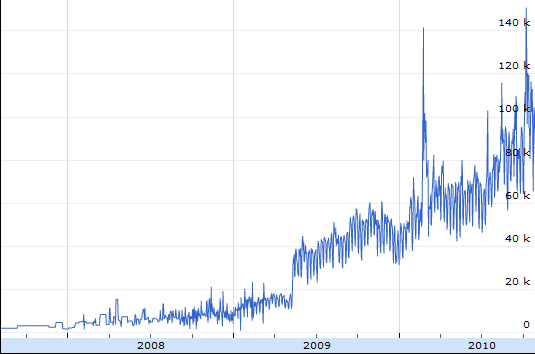
\includegraphics[width=0.9\textwidth]{cloudkick_daily_ec2_launch_counts.png}
  \caption{估测的 Amazon EC2 云平台 us-east-1 区域在 2007 至 2010 年每天的虚拟机实例启动数量 \cite{ec2dailyusage}}
  \label{figure:daily_ec2_launch_counts}
\end{figure}

没有激励云租户调整计算需求的手段,所有的计算需求可能会在同一时间堆积。如果云租户的计算需求可以被调整,将会有更大的潜力去平滑云平台中的计算资源请求。这最终可以形成对计算设备的更有效使用,提升云平台的资源使用率。虽然类似 Web 应用这类需要随时处理用户请求的实时应用很难接受这种调整,批处理任务等其它类型的应用在自身特点上是更加灵活、有弹性的。一个批处理任务通常没有时间限制或只需在一个截止期限前计算出结果就可以。这类任务可以很灵活的在计算资源可用的时候完成计算。

市场化地根据供需关系进行价格调节是非常有望促进需求转移的有效机制,云平台提供商可以通过价格信号表达云平台中当前的计算资源利用率。一个更高的价格会使可以延迟使用计算资源的云租户放弃他们当前的计算资源请求。相反地,一个更低的价格通过经济上的激励可以吸引更多的使用者。为了近一步提升计算资源利用率,IaaS 云平台提供商的旗舰 Amazon EC2 云平台已经引入了一个新的计算资源提供形式————竞价云实例。

与按需云实例不同,竞价云实例的价格根据云平台计算资源的供需关系不断变化。竞价云实例通常以极低的价格出售,但面临着随时被云平台回收的风险。当使用一个竞价云实例的时候,云租户必须首先设定一个竞价价格,作为每小时愿意支付的最大价格。竞价云实例的使用费率按每个小时开始时的竞价云实例市场价格确定。随着竞价云实例市场价格的连续波动,在该价格上升超过云租户设定的竞价价格时,云租户的竞价云实例将被关闭。直到竞价云实例市场价格升高至超过云租户设定的竞价(竞价不足失效)或者云租户主动选择关闭该节点时,该竞价云实例将结束运行。如果竞价云实例被 Amazon EC2 云平台关闭,最后不足一小时的部分将不会对云租户收取费用。如果云租户主动关闭了竞价云实例,则同使用按需云实例相同,需要支付最后不足一小时部分的费用。除了价格和可用性,竞价云实例同按需云实例是相同的。

同按需云实例一样,竞价云实例向云租户提供了足够大的实例配置类型 \cite{AWS_IT:2014} 选择空间,包括:CPU、内存、存储及网络带宽等资源的各种不同组合的硬件配置。云租户可以根据自身的应用特点和需求选择不同的实例类型。虚拟机实例分布在全球的多个地理区域 \cite{AWS_GI:2014} 中,地理区域的数量仍在继续增长中。为了保证最大程度的容错和稳定性,每个地理区域又被分成了多个隔离的空间。每个隔离的独立空间被称为一个 ``可用区''(Availability Zone)。如图 \ref{figure:aws-gi} 所示,目前 Amazon EC2 云平台有 12 个地理区域和超过 30 个可用区。本文中的应用就构建在这些可用区中,在不同可用区上的竞价云实例在价格变化和节点失效都是相互独立的。
\begin{figure}
  \centering
  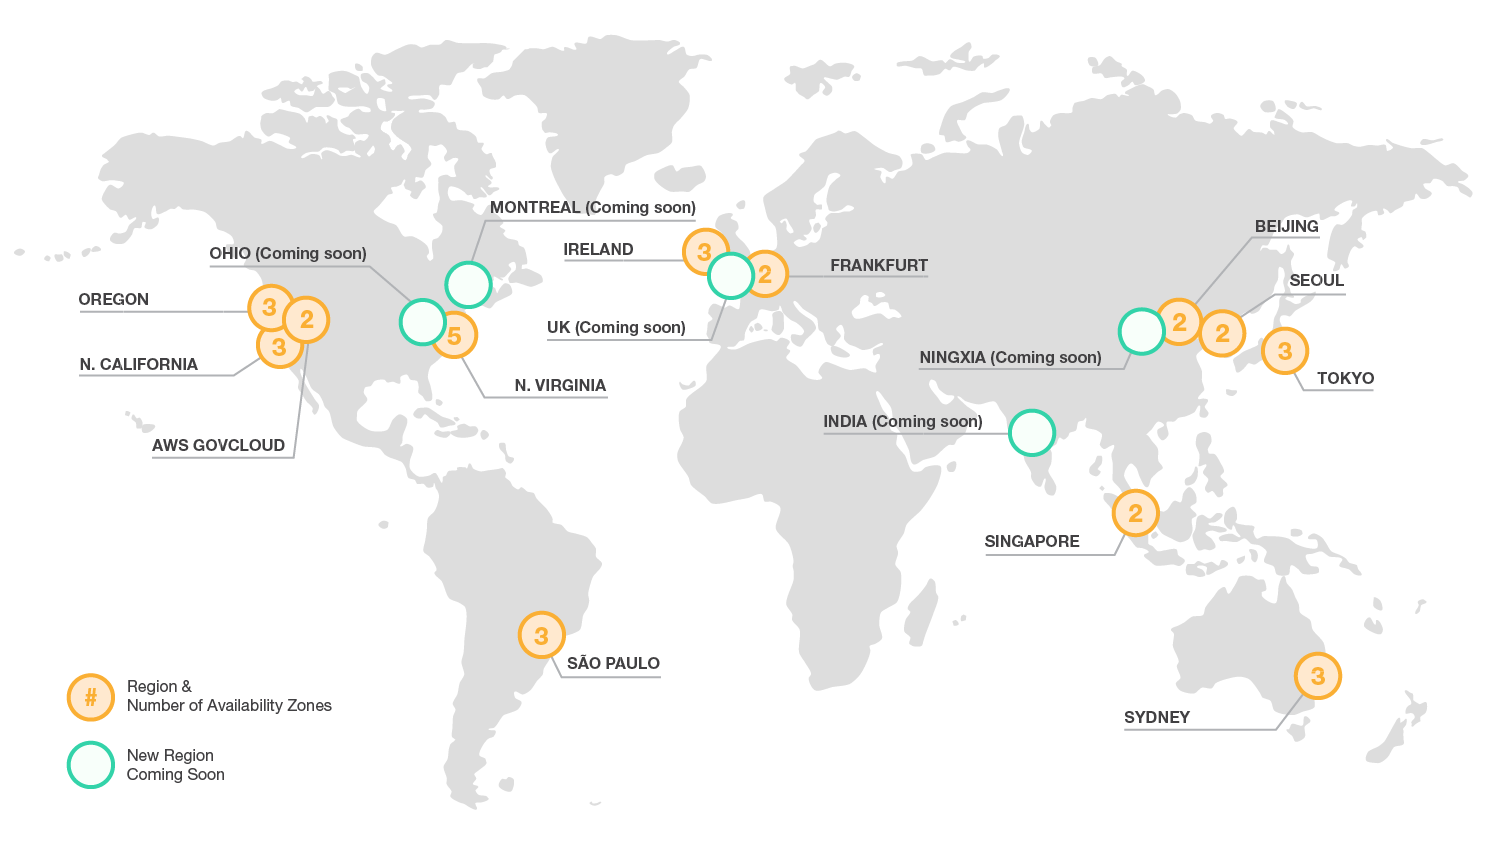
\includegraphics[width=0.9\textwidth]{Global-Infrastructure.png}
  \caption{AWS 全球基础设施地理区域和可用区概览 \cite{AWS_GI:2014}}
  \label{figure:aws-gi}
\end{figure}

要使用竞价云实例,云租户需要提交一个竞价云实例请求。在这个请求中指定实例配置类型、实例所在的可用区,以及每小时愿意支付的最大价格(被称之为 ``竞价'')。竞价云实例的市场价格由 Amazon EC2 云平台给出,价格的波动由竞价云实例资源数量的供求关系决定。图 \ref{figure:spdemo} 描述了在一段时间内竞价云实例的市场价格波动以及对某个竞价下的竞价云实例可用性的影响。当云租户给出的竞价大于等于当时的市场价格,申请的竞价云实例将启动并正常运行。显然,竞价价格设置越高竞价云实例相对越可靠、可用性越高,但又可能带来一个过高的成本。
\begin{figure}
  \centering
  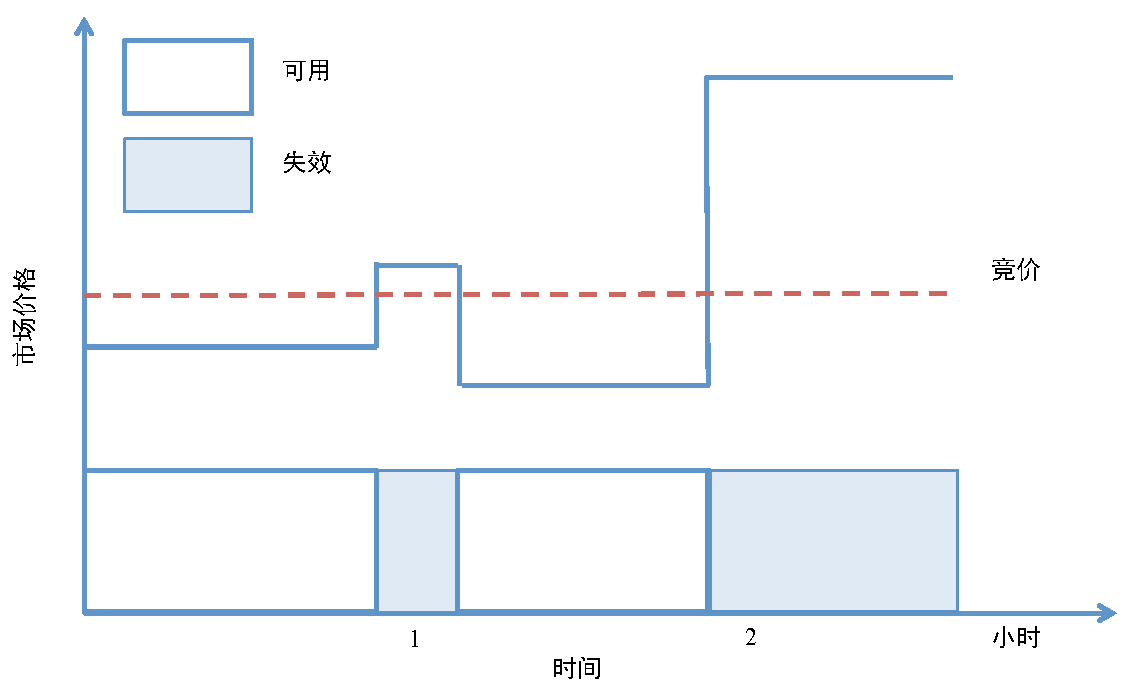
\includegraphics[width=0.85\textwidth]{spotpricedemo}
  \caption{类型竞价云实例市场价格变化示意图}
  \label{figure:spdemo}
\end{figure}

竞价云实例 \cite{SI:2014} 的出现已经给云计算带来了一个新的视野和想象空间:计算资源可以真正的如同其它商品一样在市场中根据供需关系调整价格。这对于云平台提供商来说是非常重要的一个变化:新的竞价云平台拥有了调控不同时间段计算资源使用需求的能力。对于云租户来说,通过合理设计部署在云平台中的计算应用,利用竞价云计算资源可以节省大量的计算成本。总而言之,竞价云平台的出现给云计算提供了新的活力和生机。这一变化使云平台提供商和云租户有望达成双赢的局面,并最终提高云计算资源的利用率。然而,竞价云实例本身价格波动带来的易失效特点也让云租户望而却步。直接将应用运行在竞价云实例上面临着计算的正确性、可靠性等诸多问题,而如何在不影响自身计算需求的情况下有效利用竞价云实例降低计算成本则成为了摆在所有云租户面前的一大障碍。

本文从云租户的角度出发,充分探索了竞价云平台给计算资源的使用带来的机遇和挑战。一方面利用竞价云实例有可能实现计算成本的大幅缩减,另一方面部署在竞价云实例上的应用可用性及性能得不到保障。通过对云平台中各个类型应用的分析和调研,本文认为这两方面并非是不可兼得的 ``鱼和熊掌'',而且舍弃任何一方面都将使得在竞价云平台上部署系统和应用变得毫无意义。通过对有着不同可用性要求的代表性应用有针对性地改进和设计,本文从计算机系统研究的层面给出了云租户在面对新的竞价云计算资源时如何提升在其上部署的系统的可用性及性能的方法和思路。

本研究的重要意义在于为竞价云实例的使用提供了技术基础,从而推动云租户接受、拥抱云计算的新变化。这不仅为云租户带来了大量的计算成本节约、为云平台提供商带来了计算资源使用率的提升,实现了云平台提供商与云租户的双赢。而且也间接地实现了对支撑云计算的基础设施、硬件材料、电力能源等资源的有效利用,有着深远的社会效益。

\section{面临问题与挑战}
对于云租户来说,在竞价云平台中面临的最主要问题就是如何应对竞价云实例随时可能被回收的不可靠特点。这可能导致一个正在执行的计算任务被终止造成结果数据丢失,一个正在运行的 Web 服务失效造成用户无法访问,一个分布式系统运行异常出现数据不一致。即使是利用竞价云实例作为按需云实例的补充,也可能造成系统性能的严重下降。

虽然很多系统本身有容错机制,在处理竞价云实例的节点失效上仍有不足。竞价云实例的节点失效是和市场价格以及设定的竞价相关的,这同其他的电力中断、网络拥塞、软件或硬件错误等类型故障形式极为不同,且发生频率要远高于这些常规故障。另外对于同一可用区中的两个竞价云实例来说,不论二者的竞价设定相同与否,在被回收导致的节点失效上二者是相关联的。对于需要使用大量虚拟机实例的系统来说,大量的节点关联失效也是一般容错设计上不会考虑的问题。

对于不同类型的系统来说,因各自的执行特点与需求不同,在使用竞价云实例所面临的问题与挑战也各不相同。从对竞价云实例的使用方式上,可以简单地将在竞价云平台运行的应用分为三类:1)加速任务,将竞价云实例作为性能加速器,系统中还使用可靠的按需云实例,如:大规模分布式并行处理任务;2)可中断的计算任务,如:批处理任务;3)和不可中断的、要求一直可用的服务,如:Web 服务、移动应用服务、存储服务等。具体地,又可将可中断的计算任务分为时间灵活的计算任务和有截止期限要求的计算任务两类。后者主要是那些虽没有实时性要求但超过截止期限就失去其价值的任务,如:天气预报、股票走势分析等。

对于使用竞价云实例加速大规模并行任务执行的系统,主要在于如何避免竞价云实例的加入反而拖慢了整体作业执行进度。成本和性能的权衡是在这个应用场景中主要关心的问题。如果使用竞价云实例投入的成本最终没有得到超过对应成本的按需云实例所能带来的性能提升甚至是反而带来了性能下降,那使用竞价云实例也就没有任何意义了。如:Chohan 等人 \cite{chohan2010see} 就指出:由于竞价云实例的不可靠性,直接将竞价云实例作为加速器引入一个由按需云实例组成的 MapReduce 集群可能带来负面的影响。在 MapReduce 作业执行过程中,竞价云实例节点被回收带来的相应任务重新执行会导致作业整体进度被拖慢。在这种情况下,使用竞价云实例不但无益反而有害。

运行在竞价云实例上的时间灵活、可中断的批处理任务,一般可以采用检查点等方式进行容错。但检查点或是其他容错手段一般会带来一定程度的运行时开销,以检查点为例:在批处理任务执行的某个时间点,如果不做检查点而竞价云实例被回收则会丢掉自上一个检查点到该时间点的任务进度,重新计算需要一定的计算成本;如果做检查点而竞价云实例正常运行则进行检查点的开销反而浪费了一些计算成本。如何使用、何时使用合适的容错机制是这类任务在使用竞价云实例时要解决的核心问题。有截止期限、可中断的计算任务,使用竞价云实例时需要考虑的问题则更复杂一些。一方面,虽然有截止期限但该计算任务并非要求实时处理也可以被中断,因而也可以考虑在容错和计算成本之间的权衡。另一方面,如何保证计算任务可以在截止期限之前完成也需要重点关注。

一般观点认为,不可中断的、要求一直可用的服务不应该使用竞价云实例。但实际上对于分布式服务来说,自身已经有副本状态机的容错机制可以容忍一定数量的节点错误。将这样的分布式服务部署在竞价云平台上的时候,由于节点失效模型的改变对整个分布式服务的可用性带来多大影响?可用性与计算成本之间如何权衡?这是此类本身有一定容错能力的分布式服务在竞价云平台中面临的问题。服务提供商对于成本节约的追求驱动着使用竞价云实例部署在线服务的研究,借助于竞价云平台新推出的回收告警通知特性,已经有研究者提出利用嵌套虚拟化、虚拟机活迁移等技术在竞价云实例被回收时快速切换到一个按需云实例上的方法。但如何保证在竞价云平台上在线服务仍有足够的可用性?同时是否会带来过大的性能开销?为弥补性能开销所花费的计算成本是否会超出使用竞价云实例所节约的计算成本?这些纷繁的问题对于在线服务如何利用竞价云实例提出了更加复杂且巨大的挑战。

综上,本文要解决的问题是在竞价云平台中如何根据不同类型的应用选择合适的容错机制,改进容错机制,甚至是通过对系统本身设计的修改实现在计算成本、可用性、性能三者之间的最佳平衡点。或者说在使用竞价云实例的应用节省成本的同时,如何提升各类应用的可用性和性能是本研究面临的主要挑战。

\section{研究内容与主要贡献}
\subsection{本文的研究内容}
通过对竞价云平台中相关研究现状的调研可以发现:对于可中断的计算任务如何使用竞价云实例的研究已经相对成熟,而对于包括分布式服务和在线服务在内的不可中断、要求高可用的服务如何部署在竞价云实例上的研究还十分缺乏或者是存在诸多限制。另外,MapReduce 之外的大规模计算密集型并行任务处理中如何利用竞价云实例实现性能加速也还缺少相关研究。
\begin{figure}
  \centering
  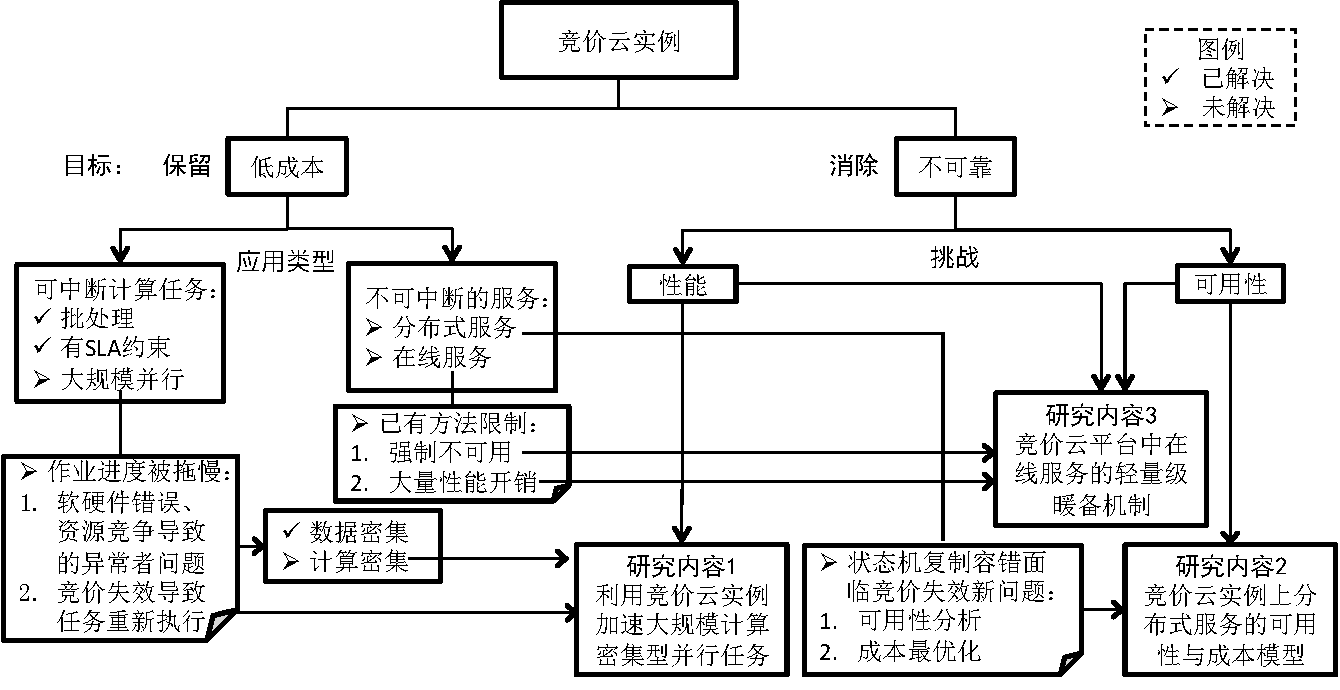
\includegraphics[width=0.9\textwidth]{proposals.pdf}
  \caption{本文研究内容概览}
  \label{figure:research_proposals}
\end{figure}

结合使用竞价云实例的各类应用所面临的不同问题和挑战,展开来说,如图 \ref{figure:research_proposals} 所示,本文的研究内容主要包括以下几个部分:
\begin{enumerate}
\item 研究如何利用竞价云平台提供的低成本计算资源加速大规模计算密集型并行任务的执行,缩减作业完成时间。这部分主要探索的是低成本的计算资源可以对大规模并行任务处理的任务调度、执行优化带来哪些变化。简单地用竞价云实例进行水平扩展可以加速作业执行,然而不可靠的竞价云实例会加剧大规模并行任务处理中的异常者拖慢整体作业进度问题。将竞价云实例用于解决异常者问题的投机执行等策略是较为恰当的使用方式,加速任务执行的同时避免了节点失效拖慢作业进度。具体地,针对一类难于预测进度的计算密集型并行任务,利用廉价的计算资源解决大规模并发时的异常者问题、加速任务执行。
\item 针对自身有容错机制的分布式服务,研究将其部署在竞价云实例上的可行性以及如何部署以达到可用性要求。由于分布式服务使用副本状态机的机制进行容错,可以容忍一部分节点失效。但竞价云实例的失效概率远高于按需云实例,使用同样多节点的分布式服务在竞价云平台中的可用性会降低很多。使用更多的竞价云实例可以提高可用性但增加了计算成本,根据此类分布式系统的可用性模型结合竞价云实例的失效特点分析分布式服务可用性与计算成本之间的关系是这部分研究的重点。
\item 基于 Amazon EC2 新推出的竞价云实例回收告警通知特性,设计在竞价云平台中提供在线服务的故障转移方法,消除现有方法的在可用性、性能上的限制。综合利用多种高可用设计和容错机制,提升竞价云平台中在线服务的可用性。减少现有方法中大量的运行时性能开销,同时在成本效率上应和现有方法的水平相当。
\end{enumerate}

\subsection{本文的主要贡献}
本文的主要贡献在于分析了竞价云平台中各类应用在计算成本、可用性、性能的潜在优化空间,探索了在使用竞价云实例的各类应用中如何提升可用性及性能,具体贡献和创新点可简要概括如下:
\begin{enumerate}
\item 针对大规模计算密集型并行计算任务中普遍存在的异常者问题,提出了基于程序跟踪和聚类分析的异常节点检测方法和基于任务克隆、投机执行、任务再分割等策略的加速执行方法。竞价云实例的使用使得这些方法在计算成本上变得可行。基于上述方法并考虑竞价云实例易失效的特点,实现了一个稳定、高效的大规模计算密集型并行任务加速器。实验评测显示该加速器在 Cap3 和 GaussianBlur 两个典型应用上可以将大规模计算密集型并行任务的作业完成时间缩减超过 20\% 和 40\%,而产生的计算成本开销只有约 3\%。
\item 指出了在竞价云平台中,分布式服务的可用性发生了较大变化。这同竞价云实例的失效特点是相关的,而竞价云实例的失效概率模型本质上是由竞价云实例的市场价格和竞价决定的。进而提出了使用竞价云实例部署分布式服务所面临的竞价决策问题的非线性规划模型,并给出了可用性和成本感知的竞价框架。该竞价框架可以在保持同按需云实例同样可用性级别的前提下大幅减少计算成本,在分布式锁服务和分布式存储服务的案例中分别得到了 81.23\% 和 85.32\% 的成本节约。
\item 提出了基于暖备对的在竞价云实例上提供在线服务的方法。这个方法消除了已有工作在可用性和性能上的限制。暖备的故障转移机制通过将服务迁移中不可控的虚拟机实例申请和启动过程移出关键路径从而消除了强制性的不可用。轻量级的迁移方法和时间可控的异步磁盘镜像极大地提高了系统性能。另外,该方法在多个地理区域、多个可用区之间从价格趋势及稳定性上综合考虑竞价策略对可用性和成本的影响。评测结果显示这个方法可以在同现有方案相近的计算成本下显著提升服务可用性和性能,在线服务的不可用性降低了接近一个数量级,在 TPC-W 和 YCSB 基准测试集上获得了至多 45\% 和 100\% 的性能提升。
\end{enumerate}

\section{全文组织结构}
本文其他各章内容组织如下:在第 \ref{cha:background} 章首先从竞价云实例的市场价格模型、利用竞价云实例执行可中断的计算任务以及如何在竞价云平台中实现高可用、高可靠等方面分析了当前竞价云实例应用优化工作的研究现状,然后对本文涉及到的子领域的相关工作做了简要介绍。在第 \ref{cha:no2} 章详细介绍了利用竞价云实例加速大规模计算密集型并行任务的方法。在第 \ref{cha:jupiter} 章形式化了在竞价云平台中部署分布式服务所面临的可用性与成本的最优化问题,并给出了综合考虑成本与可用性的竞价框架设计。在第 \ref{cha:gemini} 解释了现有利用竞价云实例提供在线服务的方法在可用性和性能上存在的诸多限制,提出了一个基于暖备的在竞价云平台上提供在线服务的轻量级容错机制。最后,在第 
\ref{cha:conclusion_futruework} 章总结了本文工作并对未来工作进行了展望。

\chapter{研究现状和相关工作}
\label{cha:background}

本文的全部工作都是针对竞价型云平台相较传统云平台的新特点对几类典型系统应用的模型和设计加以改进以提升其性能与可用性,在整个研究工作中涉及到多个不同的子领域。本章首先对竞价型云平台的研究现状尤其是竞价型实例应用优化工作进行详细介绍和分析,然后再对本文的研究中所涉及的子领域相关工作加以讨论。

针对竞价型云平台的研究工作主要包括竞价型实例的市场价格预测模型、适应竞价型实例的计算框架设计、在线服务架构等等。竞价型云平台的出现时间比较短,竞价型实例价格动态变化的特点是传统云平台中的应用不曾考虑的。竞价型实例的市场价格预测模型为更好的认识和使用竞价型实例提供了基础支持和帮助。新型的计算资源有着极其诱人的低廉价格,随之而来的是随时可能被云平台回收的不可靠属性。如何利用这些竞价型实例实现效益可观的计算成本节省,同时保证应用的可用性及性能?通常的观点认为:竞价型实例的自身特点决定了它只适合使用在不需要高可用性的场景中。大部分研究工作也是针对可中断、时间相对灵活的计算任务考虑如何利用竞价型实例实现计算成本的最大节约,以及设计应对竞价型实例特有的节点失效的容错手段。但计算成本节约上的巨大经济驱动力推动着竞价型实例向其它场景的普及,已经有一些工作开始尝试利用竞价型实例提供高可用的在线服务。甚至有研究者设计出将不可靠的竞价型实例封装为可靠计算资源的初步方案。

本文还涉及到的多个不同子领域包括:大规模并行任务调度、分布式系统可用性理论、高可用及迁移技术等。这些相关领域的工作有的为本文提供了参考和帮助,有的是本文的方法和技术得以实现的基础。但本文所面临的是充满挑战的新问题,需要在新的背景和环境下重新审视已有方法和技术并作出创造性的改变。本章在讨论这些相关工作时,将结合本文要解决的问题进行详细说明。

\section{竞价型实例的市场价格模型}
考虑到部署在竞价型实例上的计算系统的调度算法和容错机制设计的需要,竞价型实例价格预测是一个相关研究中需要探索的基础问题。竞价策略的设计和竞价型实例的失效模型都离不开对市场价格的预测分析。虽然 Amazon EC2 等云平台并没有披露其底层定价算法的细节,许多研究者在云平台外部对竞价型实例的价格模型进行了深入研究。

Javadi 等人 \cite{Javadi:2011:SMS:2120969.2121740} 对 Amazon EC2 云平台的四个区域一年多的市场价格历史数据做了全面的统计分析。基于对所有配置类型竞价型实例的价格和价格变化间隔时间的详细分析,Javadi 等人认为竞价型实例的市场价格数据有明显的双模态性,而竞价型实例的价格变化间隔则在两小时处形成明显的峰值。而且除了 m1.small 类型竞价型实例,竞价型实例市场价格的概率分布是几乎对称的。m1.small 类型实例的不同可能是作为 Amazon EC2 云平台中最便宜的计算资源有着同其它类型节点不同的使用模式造成的。据此,他们提出了使用如下的高斯混合分布来拟合竞价型实例的价格和价格变化时间间隔的概率统计模型如式 \eqref{eq_mog} 。
\begin{equation}\label{eq_mog} 
CDF(x; k, \vec p, \vec u, \vec{\sigma^2}) = \sum_{i=1}^{k}{\frac{p_i}{2}(1+erf(\frac{x-\mu_i}{\sigma_i\sqrt{2}}))}
\end{equation}

其中 $\vec u$,$\vec{\sigma^2}$,和 $\vec p$ 是 $k$ 个高斯分布的均值、方差和概率的向量。而 $erf$ 是误差函数,定义如下:
\begin{equation}\label{eq_erf}\nonumber 
erf(x) = \frac{2}{\sqrt{\pi}}\int_{0}^{x} e^{-t^2}dt
\end{equation}

通过参数估计和模型校准,该模型在新的价格数据集上的最大相对误差小于 4\%。该模型为深入的理解竞价型实例的市场价格提供了一个良好的基础,但该模型没有考虑用户的竞价对竞价型实例的节点失效的影响。

Ben-Yehuda 等人 \cite{AgmonBen-Yehuda:2013:DAE:2509413.2509416} 推测截止2011年10月之前 Amazon EC2 云平台的竞价型实例的市场价格在大部分时间内并不是市场驱动的,而是由一个云平台内部的基于自回归模型的定价算法确定的。通过对大量竞价型实例历史价格数据的分析,Ben-Yehuda 等人认为在较高的价格时反映了市场变化、在较低的价格时则是决定于一个动态保留价格。该动态保留价格通过一个隐藏的一阶自回归模型随机设定。对于式 \eqref{eq_ar1} 所示的一阶自回归过程:
\begin{equation}\label{eq_ar1} 
\Delta_i = - a_1\Delta_{i-1}+\epsilon(\sigma)
\end{equation}

2010 年 4 月 到 7 月的竞价型实例价格数据可以拟合的非常好(即:更高阶的 $a_i, i > 1$ 的系数可忽略)。其中,$a_1 = 0.7$,$\epsilon(\sigma)$ 是标准差为 $\sigma$ 的白噪声。令 $F$ 和 $C$ 分别表示人为指定价格范围的下界和上界,$\sigma$ 的拟合结果为 $0.39 (C - F)$。这个拟合结果在大多数实例类型上都得到了准确验证。唯一的例外也是 m1.small 类型的竞价型实例,该类型下的拟合结果是 $a_i = 0.5$,$\sigma = 0.5 (C - F)$。基于这些分析和数据拟合,Ben-Yehuda 等人构造出的保留价格算法主要步骤如下:
\begin{enumerate}
\item 将保留价格 $P_0$ 初始化为 $F$,价格变化 $\Delta_0$ 初始化为 $0.1 (C - F)$。
\item 下一个保留价格 $P_i$ 由 $P_{i-1} + \Delta_i$ 给出,其中 $\Delta_i = - 0.7 \Delta_{i-1}+\epsilon(0.39 \cdot (C - F))$。
\item 如果 $P_i \notin [F, C]$,则重复执行上一步骤。
\end{enumerate}

F 和 C 根据虚拟机实例类型各不相同,价格最终需要四舍五入保留精度到 0.1 美分。他们的研究工作给竞价型云平台的相关研究尤其是使用竞价型实例的价格数据的研究工作一个非常重要的提示:在对价格数据的分析中一定要区分这部分数据是由云平台的内部机制随机设定的,还是真正的反映了真实的市场供需关系。以 2011 年 10 月之前的竞价型实例价格数据为例,很多价格数据特征(最小值、变动间隔等)表现出明显的人工干预行为。最后他们提醒其它研究者在进行竞价型实例价格预测模型训练时,一定要注意使用的价格历史数据的时间节点。

Chohan 等人 \cite{chohan2010see} 和 Song 等人 \cite{song2012optimal} 通过统计推断确认了 Amazon EC2 云平台的竞价型实例的竞价价格序列满足马尔科夫性,Song 等人指出竞价型实例的价格变化时间间隔并不满足无记忆型。根据 Sewook Wee \cite{5948651} 在 2011 年的分析,竞价型实例市场价格采样累计分布函数约每一个小时有明显的增长。Song 等人在他们的工作中将竞价型实例的历史价格数据被以 1 小时为单位做离散化处理,并使用一个离散化的半马尔可夫(semi-Markovian)链描述竞价型实例的价格波动。

这个马尔可夫链的边是以 1 小时为间隔的价格转移概率。给定概率转移矩阵,可以使用如下的 Chapman-Kolmogorov 等式的变体式 \eqref{eq_ck} 计算 $n$ 步转移概率:
\begin{equation}\label{eq_ck} 
P(i, b, n) = \sum_{j \notin B}{M_{ij}P(j, b, n-1)}
\end{equation}

其中初始概率由式 \eqref{eq_ckcond} 给出,
\begin{equation}\label{eq_ckcond} 
P(i, b, 0) = 
\begin{cases}
0 &\mbox{if $i \in B$}\\
1 &\mbox{if $i \notin B$}
\end{cases}
\end{equation}

其中,竞价型实例在启动时的初始市场价格为 $i$,经历了 $n$ 个时间单元。超过竞价 $b$ 的价格的集合为 $B$。$M_{ij}$ 是价格点 $i$ 到价格点 $j$ 的转移概率矩阵。$P(i, b, n)$ 可以通过递归的方式求解。最基本的转移概率(第 0 步转移概率)就是判断所设定的竞价能否申请到竞价型实例。

在本文的关于使用竞价型实例的分布式服务的可用性与成本模型的工作中,半马尔可夫(semi-Markovian)链模型被嵌入到竞价型实例的失效模型中。

\section{竞价型云平台上执行可中断计算任务的方法}
自 Amazon EC2 发布竞价型实例以来,相关领域的研究人员已经表现出了对利用竞价型实例实现低成本计算的极大兴趣。考虑到竞价型实例可能因竞价不足失效的特点,大部分现有工作集中于将竞价型实例用于可中断、时间灵活的计算任务。研究的对象包括主流计算框架 MapReduce、批处理任务、有截止期限或 SLA 要求的任务等。其中有些研究工作主要考虑的是在一个固定竞价下如何解决竞价型实例的频繁失效问题,有些研究工作则基于统计分析和竞价型实例市场价格历史数据设计动态竞价策略。

\subsection{MapReduce 作业}
Chohan 等人 \cite{chohan2010see} 基于对竞价型实例市场价格序列满足马尔科夫性的分析,给定当前的竞价型实例市场价格 $i$,竞价 $b$,最大执行时间单元数 $\tau$,可以得出该竞价型实例的寿命 $l$ 的期望可表示为式 \eqref{eq_elife} 。
\begin{equation}\label{eq_elife} 
E(l) = \sum_{n=1}^{\tau}nP(i, b, n)
\end{equation}

此模型可以用于有计划的备份数据减少竞价型实例失效带来的损失,而且可以用于竞价策略保证在相同的计算成本预算下获得更多的竞价型实例。Chohan 等人通过实验证明了使用竞价型实例可以有效加速 MapReduce 任务的执行,对于某些任务可加速超过两倍而计算成本只有 44\%。同时,一些测试中也出现了相比不用竞价型实例变慢了 27\% 的情况。

MapReduce 计算框架中的容错机制可以处理竞价型实例被回收的情况,但可能增加 MapReduce 作业的完成时间。Chohan 等人的工作通过对竞价型实例市场价格的建模和实验验证揭示了使用竞价型实例加速时间灵活、可被中断的计算任务的机会。

对于使用竞价型实例的 Hadoop \cite{hadoop:2014} 计算框架,一个任务的失败不会导致整个作业的执行失败。失败的任务可以被调度到其它可用的竞价型实例或按需型实例上重新执行。只要将记账任务(bookkeeper)部署在正常的按需型实例上保证他在作业执行期间不间断的运行,整个作业中的所有任务最终会得以调度和完成。然而,Hadoop 等许多 MapReduce 实现中并没有考虑为竞价型云平台作出针对性的设计。为了能真正利用到竞价型实例的低成本优势,Huan Liu \cite{Liu:2011:CMC:2170444.2170450} 在其之前的工作 Cloud MapReduce \cite{Liu:2011:CMM:2007336.2007355} 的基础上提出了 Spot Cloud MapReduce。

Cloud MapReduce 的特点是使用了多种云平台服务,如:Amazon EC2 云平台的 S3 (Simple Storage Service),SQS (Simple Queue Service),SimpleDB (Simple Database Service),大大简化了 MapReduce 计算框架的设计。在 Cloud MapReduce 中,一个 MapReduce 作业的输入文件存放在 S3 中。通过 SQS 创建多个队列(Map 队列,Reduce 队列,Master 队列,Output 队列)用于控制作业进行,Reduce 队列有多个,其它队列各有一个。执行 Map 任务的虚拟机实例从 Map 队列获取要处理的文件位置,从 S3 读取文件,将结果放入 Reduce 队列。执行 Reduce 任务的虚拟机实例从 Master 队列获取要处理的数据位置,从 Reduce 队列读取中间数据,将结果写入 Output 队列。执行 Map 任务和 Reduce 任务的虚拟机实例在完成任务后,向 SimpleDB 提交完成记录,这样通过查询 SimpleDB 就可以判断整个作业进行到哪个阶段、是否完成。

为了应对竞价型实例带来的 Cloud MapReduce 作业的大量工作节点失效问题,Spot Cloud MapReduce 基于 Cloud MapReduce 做出了如下改变:
\begin{enumerate}
\item 修改了 Map 队列中任务划分的格式,除 Map 任务的 id,对应文件位置外,还加入了文件的偏移。对于作业初始划分,文件偏移均为 0。
\item Spot Cloud MapReduce 实现了 Map 任务的流式输出到分级缓冲区,并尽快持久化到 Reduce队列。当竞价型实例被回收时,Spot Cloud MapReduce 利用关机脚本做应急处理,首先停止用户定义 Map 函数的执行,然后将分级缓冲区中的数据提交到 Reduce 队列中。
\item 在任务提交机制上改为允许部分提交,即:当分级缓冲同步到 Reduce 队列后,记录该 Map 任务的对应文件偏移部分已处理完。
\item 最后只要在 SimpleDB 中查询到一个任务的输入文件的所有对应部分,就表示该任务已完成。如有缺少的部分,则重新在 Map 队列中加入新的任务处理该部分输入。
\end{enumerate}

由于 Amazon EC2 的 SQS 不支持 FIFO,Reduce 任务无法实现流式输出到 Output 队列。Spot Cloud MapReduce 只修改了 Map 任务部分的实现,这已经能够在很大程度上保证大量节点同时失效的情况下计算任务继续执行下去并最终得以完成。通过使用竞价型实例,执行 MapReduce 作业的成本将会大大降低。当然,MapReduce 作业的完成时间可能变得很长。

通过直接修改系统本身的实现,Spot Cloud MapReduce 无需借助任务检查点等手段就达到了容错的目的。对于类似的可以直接修改实现的系统,在检查点需要保存的数据量比较大的情况下,这是在利用竞价型实例时应首先考虑的一个更为高效的实现思路。

\subsection{批处理作业}
针对计算密集型的、任务可分的批处理作业,Yi 等人 \cite{Yi:2010:RCS:1844768.1845343, 5975137} 提出了自适应的检查点策略和实例类型切换策略来尽量消除使用竞价型实例带来的不可靠,减少作业执行成本和作业完成时间。检查点技术是将当前应用全部状态的快照写到一个持久化存储设备中,在之后的某个时间点遇到故障时通过使用之前的快照恢复执行的容错机制。Yi 等人研究了在竞价型云平台的场景中何时做检查点最优的策略问题。

在Yi 等人设计的自适应检查点策略中,每十分钟进行一次是否要做检查点的决策。这个决策基于在这之后发生竞价节点失效时的所需预期恢复时间 $R(t)$。可以分别计算在跳过这个检查点和做这个检查点的情况下发生竞价节点失效时所需预期恢复时间 $R_{skip}$,$R_{take}$。如果 $R_{skip} > R_{take}$,则应该做这个检查点,否则应该跳过这个检查点。$R_{skip}$ 和 $R_{take}$ 的预估依赖于基于已有价格历史数据做出的概率统计,用于计算的其它参数有原始竞价价格,已经正常运行的时间,上次检查点到现在的时间,以及现在的竞价型实例市场价格。

令 $t_p$ 表示当前时间点,$t$ 表示上次做检查点距 $t_p$ 的时间长度,$t_r$ 表示完成作业相对 $t_p$ 还需的时间长度,$r$ 表示节点失效后重启一个任务所需的时间开销,$t_c$ 表示做检查点之间的时间间隔,$f(t)$ 表示在给定竞价价格和当前市场价格下经过时间 $t$ 节点的失效概率,$T(w, t_p)$ 表示在没有检查点的情况下,从时间点 $t_p$ 开始完成一个需要在 $w$ 个时间单元不出现节点失效的任务所需的期望执行时间,则 $R_{skip}$ 和 $R_{take}$ 可分别表示为式 \eqref{eq_rskip} 和 \eqref{eq_rtake} 。
\begin{equation}\label{eq_rskip} 
R_{skip}(t, t_p) = \sum_{k=0}^{t_r - 1}(k + r + T(t,t_p))f(k+t_p)
\end{equation}
\begin{equation}\label{eq_rtake} 
R_{take}(t, t_p) = \sum_{k=0}^{t_r - 1}(k + r)f(k+t_p) + t_c\sum_{k=t_r}^{\infty}f(k+t_p)+T(t,t_p-t)\sum_{k=0}^{t_c - 1}f(k+t_p)
\end{equation}

其中 $T(w, t_p)$ 如式 \eqref{eq_t} 所示,
\begin{equation}\label{eq_t} 
T(w,t_p) = \frac{w\sum_{k=w}^{\infty}f(k+t_p)+\sum_{k=0}^{w-1}(k+r)f(k+t_p)}{1-\sum_{k=0}^{w-1}f(k+t_p)}
\end{equation}

对于可分的任务负载(应用本身可以灵活根据 CPU 核心数运行)面临竞价型实例被回收时,Yi 等人认为可以考虑选择其它不同配置类型的竞价型实例并提出了实例类型切换策略。在Yi 等人提出的节点配置类型切换策略中,主要提供了如下启发式规则:
\begin{enumerate}
\item 最低价:选择按每核价格计算最低的实例类型。直觉上似乎某个类型的竞价型实例市场价格越低,再相同竞价下出现竞价不足的可能越小。
\item 最低失效概率:选择失效概率最低的实例类型。失效概率的分布根据价格数据动态计算,最低失效概率考虑了设定的竞价、竞价型实例的市场价格及变化趋势。这个策略以缩短作业完成时间为目标。
\item 最高失效概率:选择失效概率最高的实例类型。失效概率越高,有更高的概率利用到不足一小时竞价型实例被回收免费的特性。这个策略的目标是减少完成作业的计算成本。
\end{enumerate}

检查点技术是计算任务常用的容错技术手段,节点类型切换策略属于竞价策略的范畴。Yi 等人的研究通过对检查点开销和出现错误的恢复时间代价上的权衡,给出了利用竞价型实例运行批处理作业时一个自适应的检查点执行策略。节点类型切换策略则从减少作业完成时间和减少作业计算成本两个角度给出了不同的启发式规则。他们的工作为如何在易错的竞价型实例上执行批处理作业的用户提供了有益参考,但他们并没有在真实系统中实现这样的策略而是通过仿真加以验证。

Subramanya 等人 \cite{Subramanya:2015:SBC:2806777.2806851} 设计实现了一个竞价型云平台中的批处理计算服务 SpotOn。SpotOn 无需对应用做出修改即可通过多种容错机制和可用区选择策略自动地消除竞价型实例被回收的影响。SpotOn 的原型实现在 Amaon EC2 上,作业被打包进 Linux 容器 \cite{LXC} 以利用高效的进程级检查点和迁移技术。根据批处理作业的预期执行时间和资源使用需要,SpotOn 在所有竞价型及按需型实例市场中选择合适的可用区和容错机制以减少作业预期完成时间。在竞价型实例被回收时,SpotOn 将在另一个可用区继续执行该作业,根据容错机制和作业资源使用的不同造成的时间开销也不同。

SpotOn 可选的容错机制和模型包括:
\begin{enumerate}
\item 被动迁移:当收到竞价型实例回收告警通知时,将作业所在容器迁移到另一个可用区的虚拟机实例上。如果在两分钟告警时间内未能完成迁移,则需在另外的虚拟机实例上重新执行该作业。这个风险的大小同需要迁移的内存和磁盘状态的大小相关。
\item 主动检查点:定期的对作业状态(包括内存和本地存储等)做检查点,这个机制没有对作业的内存工作集和本地磁盘更新大小的限制。但定期的检查点引入了一定的执行开销。
\item 复制执行:在多个可用区的多个竞价型实例执行同一个作业。复制执行的优势是不受作业的内存工作集和本地磁盘更新大小限制,并且支持并行作业。但仍然存在所有副本节点同时被回收的可能,另一个演化出的策略是在按需型实例上同时备份多个竞价型实例上执行的作业(只备份一个竞价型实例上的作业则没有使用竞价型实例的意义)。虽然这会导致在按需型实例上执行的作业副本进度变慢,但在某一个竞价型实例失效时避免了从头开始执行作业。
\end{enumerate}

SpotOn 首先根据作业特点和用户需求过滤掉不可行的容错机制,再根据各个可用区市场历史价格数据计算出不同的容错机制在各个可用区的计算成本期望 $E(C_k)$ 和作业完成时间期望 $E(T_k)$,然后选择 $\frac{E(C_k)}{E(T_k)}$ 最小的容错机制和可用区。在竞价策略上,Spoton 会确保该作业使用的竞价型实例的竞价总和不超过使用相应按需型实例的价格。

相比已有工作,Subramanya 等人给出了更丰富的批处理作业容错方式,同时实现了一个原型系统,验证了各种容错机制的可行性。采用虚拟容器的方式也保证了该方法广泛的适用性。

\subsection{有 SLA 约束的任务}
在提交某些计算任务时,用户可能还有对截止期限的要求,以及其它的 SLA 约束,如:计算成本预算。对于这类有 SLA 要求且为计算密集型、易并行、可分的任务在竞价型实例上的执行,Andrzejak 等人 \cite{Andrzejak:2010:DMC:1906481.1906533} 使用一些随机变量描述这类计算任务的执行模型:
\begin{enumerate}
\item 执行时间 $ET$:完成计算任务所需时间(包括被中断的时间)
\item 可用时间 $AT$:竞价型实例在任务执行过程中可用的时间
\item 价格期望 $EP$:竞价型实例在可用阶段平均每小时收取的费用。$EP \leq u_b$ 总是成立,$u_b$ 为用户指定竞价。
\item 计算成本 $M$:用户为每个竞价型实例支付的费用,$M = EP \cdot AT$
\end{enumerate}

一些可能的 SLA 约束如下:
\begin{enumerate}
\item 计算成本预算 $B$:每个竞价型实例所花的成本上限;且用户期望满足这个约束的可信系数达到 $C_B$
\item 截止期限 $t_{dead}$:完成任务所需执行时间的上限;且用户期望满足这个约束的可信系数达到 $C_{dead}$
\end{enumerate}

通过使用竞价型实例的历史价格数据预先计算各个随机变量的累积概率分布,可以根据如下模型给出可行的可用区选择和竞价决策:
\begin{enumerate}
\item 计算成本预算约束以可信系数 $C_B$ 被满足 $\iff B \geq M(C_B)$
\item 截止期限约束以可信系数 $C_{dead}$ 被满足 $\iff t_{dead} \geq ET(C_dead)$
\end{enumerate}

Andrzejak 等人提供了对有 SLA 约束的计算任务在竞价型实例上执行的一个简单思路,但由于所有随机变量的概率分布都是预先计算出的,对于市场价格频繁波动的情况并不适用,可能会造成 SLA 约束无法满足的情况。

从一个云服务中间商的角度考虑,Song 等人 \cite{song2012optimal} 提出了一个基于 Lyapunov 优化技术的考虑整体效益的动态竞价算法。在这个场景中,中间商接受来自云用户的作业提交请求,利用竞价型实例完成这些作业。所有作业请求都按顺序处理,这里对作业的类型限定为计算为主、可被中断,如:大数据分析(Hadoop作业)、科学计算批处理作业、生物数据处理等适合竞价型实例的。令第 $m$ 个作业的大小(即第 $m$ 个用户所需的计算量)为 $L_m$,其中 $L_m \leq L^{MAX}, \forall m$。这里 $L_m$ 是一个随机变量,但其概率分布不为中间商所知。定义 $T_m$ 为完成作业 $m$ 所需的时间,$C_m$ 为完成作业 $m$ 所需的成本。假设中间商向用户收取的费用为 $R(L_m)$,$R(.)$ 为一个任意的有届函数。则有中间商执行作业 $m$ 得到的单位时间净利润为 $(R(L_m) - C_m)/T_m$。中间商的最大化平均收益的问题可以形式化表达为式 \eqref{eq_max_profit}, \eqref{eq_cost}, \eqref{eq_eff}。
\begin{equation}\label{eq_max_profit} 
\max \lim_{M \rightarrow \infty}{\frac{\sum_{m=1}^M(R(L_m)-C_m)}{\sum_{m=1}^MT_m}}  
\end{equation}
s.t.
\begin{equation}\label{eq_cost} 
\lim_{M \rightarrow \infty}{\frac{\sum_{m=1}^MC_m}{\sum_{m=1}^MT_m}} \leq \alpha 
\end{equation}

\begin{equation}\label{eq_eff}
\lim_{M \rightarrow \infty}{\frac{\sum_{m=1}^ML_m}{\sum_{m=1}^MT_m}} \geq \beta 
\end{equation}

Song 等人指出由于模型中的 $L_m$ 的概率分布无法确定,因此应考虑设计一个在线竞价策略解决该问题。基于排队论对这一服务模型进行分析,他们使用 Lyapunov 优化技术给出了一个近似最优的收益最大化动态竞价算法。该模型具有非常良好的扩展性,可以非常方便的加入用户的一些 SLA 约束,例如:用户要求作业在一个置顶的截止时间之前完成,则可以在模型中加入约束 $T_m < D_m$ 即可。其中,$D_m$ 为 作业 $m$ 的截止期限。

Song 等人的工作分析了竞价型实例的价格模型,从云服务中间商的角度给出了一个如何利用竞价型实例处理用户提交的作业请求实现收益最大化的模型和动态竞价算法,该模型还可以方便的扩展加入用户对作业截止时间的要求。这个工作在数学模型的层面上对竞价型实例的价格变化和计算成本与作业完成时间的权衡进行了深刻诠释。

\section{竞价型云平台中实现高可用的设计}
\subsection{竞价型云平台上的高可用服务框架}
上一节介绍的所有研究工作都集中于时间灵活的、可中断的计算任务,这些计算任务的特点是可以轻松地切换到竞价型计算资源可用的时候再继续执行。这对于需要随时响应请求,不可中断的服务来说是不可能做到的。

最近,已经开始有研究者关注如何使用竞价型实例提供高可用服务这个问题。He 等人 \cite{He:2015:CCH:2749246.2749275}  提出了一个使用竞价型实例提供在线服务的解决方案。该方案大幅降低了提供在线服务的成本,通过使用嵌套虚拟化和虚拟机迁移技术来保证竞价型实例被回收时在线服务的可用性。

该方案需要在申请的竞价型实例上运行一个嵌套的虚拟机管理器(VM Hypervisor),以利用虚拟机迁移技术实现在线服务的无缝迁移。其使用的云平台上的嵌套虚拟化实现是 XenBlanket \cite{Williams:2012:XVO:2168836.2168849},但由于没有底层虚拟机管理器提供的硬件虚拟化支持接口,XenBlanket 的运行开销很大。尤其是计算密集的程序,运行时开销至多达到 68\%。 运行在线服务的嵌套虚拟机需要定期执行内存检查点任务,将内存快照存储到网络接入的 EBS 存储卷上。利用竞价型实例被回收时的告警时间,可以将最后一次内存检查点之后的更新同步到持久化的 EBS 上。由于应急处理的时间只有两分钟,这个方案使用了一个时间可控的内存检查点机制 \cite{Singh:2013:YEG:2482626.2482642}。该内存检查点机制在给定可用时间限制 $\tau$ 的情况下,通过动态调节后台检查点执行频率来保证内存状态的更新量不会超过一个阀值,即能够在时间 $\tau$ 内将全部更新写到持久化存储。由于告警时间短暂,这个方案要求嵌套虚拟机在运行过程只使用持久化的 EBS。这对于需要高 IOPS 的在线服务来说是一个很严重的问题。另外为减少迁移过程中的停机时间,该方案还使用了延迟虚拟机恢复技术。

在竞价策略方面,He 等人提出了被动策略(reactive)和主动策略(proactive)两个竞价方式。被动策略将竞价设为同类型按需型实例的价格。当竞价型实例的价格超过了按需型实例的价格,必须立即申请一个新的按需型实例。当新的虚拟机实例启动后,运行在线服务的嵌套虚拟机被强制迁移到这个新申请的按需型实例上。主动策略则将竞价设为高于同类型按需型实例的价格(以 $k$ 倍于同类型按需型实例的价格设定竞价,$k > 1$)。当竞价型实例的价格超过了按需型实例但没有超过竞价时,可以申请一个按需型实例。在这个按需型实例启动后,可以按计划将运行在线服务的嵌套虚拟机迁移到按需型实例上。如果竞价型实例的价格直接超过了竞价,处理方式则和被动策略相同。主动策略的优势在于存在一定概率避免在竞价型实例被回收时进行强制迁移。当竞价型实例的价格重新降回按需型实例价格以下时,运行在按需型实例上的嵌套虚拟机可以按计划迁移回新申请的竞价型实例。在可用区的选择策略上,He 等人给出的策略是一个简单的贪心策略。该策略直接选择多个可用区中竞价型实例的市场价格最低的。

He 等人的工作对在竞价型云平台上提供在线服务进行了积极地尝试,为实现在线服务的可用性 SLA 给出了一个值得借鉴的思路。但这个方案存在强制迁移带来的服务不可用,嵌套虚拟化带来的大量性能开销,以及无法使用高性能的本地存储等问题。本文的竞价型实例上在线服务的轻量级暖备机制正是致力于解决该工作在服务可用性和性能上的巨大限制。

\subsection{竞价型实例的可靠计算资源封装}
Sharma 等人 \cite{Sharma:2015:SDD:2741948.2741953} 站在云平台经销商的角度,从一个更基础的层面考虑可用性和可靠性。他们设计实现了一个基于竞价型云平台的导出云平台 SpotCheck,创造性地在不可靠的计算资源上向云租户提供可靠的计算资源。嵌套虚拟化技术和虚拟机迁移机制也被引入用于隐藏底层频繁的竞价型实例失效。

在保障可用性、可靠性上,SpotCheck 所使用的方法同 He 等人基本相同。所涉及到的技术也同样是:云平台上的嵌套虚拟化实现 XenBlanket,虚拟机活迁移技术、时间可控的内存检查点机制,以及延迟虚拟机恢复技术。

在架构上,SpotCheck 维护多个虚拟机实例资源池,通过嵌套虚拟机的形式向用户提供同样是 IaaS 形式的计算资源。在 SpotCheck 的多个虚拟机实例资源池中,有竞价型实例的资源池,也有按需型实例的资源池。另外,SpotCheck 还拥有一个由按需型实例组成的备份服务器池。备份服务器主要用于改善竞价型实例的内存检查点性能,内存检查点数据无需写到远程的磁盘上只需发送给备份服务器即可。通过使用备份服务器还有机会优化最终写入磁盘的数据量,减少大量不必要的 I/O 开销。多个竞价型实例复用一个备份服务器大幅降低了成本,使得利用备份服务器为竞价型实例提供高效的内存检查点机制变得可接受和实用。

还有一个需要多加考虑的是网络问题。当嵌套虚拟机发生迁移时,为了避免已经建立的网络连接不丢失需要同时实现网络 IP 地址的切换。由于底层虚拟机管理器不知道嵌套虚拟机的存在,嵌套虚拟机不能通过在网络中广播 ARP 包的方式通知他的新位置。通过在云平台的虚拟机实例中添加多块网卡并为每个网卡分配一个 EIP 地址,将不同 EIP 地址通过 NAT 机制映射到不同的嵌套虚拟机,SpotCheck 实现了嵌套虚拟机对外界的可见。在嵌套虚拟机进行迁移时,SpotCheck 通过 Amazon API 将 EIP 地址从原来的宿主虚拟机切换到新的宿主虚拟机,同时维护嵌套虚拟机管理器的 NAT 配置。

对于一个用户申请虚拟机实例的请求,SpotCheck 可以简单的在底层云平台中申请一个同样类型的竞价虚拟机实例,配置一个嵌套虚拟机提供给用户。也可以考虑申请一个配置类型更大的虚拟机,在其上运行嵌套虚拟机提供给多个用户。默认情况下,SpotCheck 使用一个贪心的策略申请竞价型实例。如果单位计算能力最便宜的实例类型恰好是用户请求的类型,则直接申请该类型。如果存在单位计算能力最便宜但实例类型更大的竞价型实例则申请该类型在其上启动一个用户需要的配置类型的嵌套虚拟机,剩余的计算能力用于提供给之后的用户申请。另外一个策略是考虑价格的稳定性,一个稳定的可用区和竞价型实例类型可以减少被回收的风险,因而减少强制迁移从而提高嵌套虚拟机的可靠性。

另外,SpotCheck尽量将用户的虚拟机请求分散到多个虚拟机实例资源池中。因为各个虚拟机实例资源池是独立的,这能减少在某个虚拟机实例资源池被回收时嵌套虚拟机迁移的数量。在为嵌套虚拟机设定备份服务器时,SpotCheck 尽量将同一个虚拟机实例资源池的嵌套虚拟机分配给不同的备份服务器。因为在某个虚拟机实例资源池被回收时,如果其中大量的嵌套虚拟机使用相同的备份服务器将对其造成巨大的请求压力。SpotCheck 使用了简单的 round-robin 策略进行备份服务器分配。在竞价的策略上,SpotCheck 同 He 等人的被动策略和主动策略相同。

SpotCheck 提供了一个非常创新的利用竞价型实例的思路,通过对底层竞价型实例的封装并使用一系列高可用、容错机制,实现了对竞价型实例的节点失效的隐藏得以向用户提供可靠计算资源。由于云平台上的嵌套虚拟化的缺陷以及回收告警时间的限制,SpotCheck 在系统运行时开销和维护可用性上的计算成本开销都比较大。尽管有一定的局限性,Sharma 等人的工作仍有很大意义,为竞价型云平台的相关研究提供了有益的参考和启发。

\section{大规模并行任务调度方法}
分布式系统中的并行任务分配与调度策略是一个被广泛研究的经典问题。在不同的场景和多变的需求下,早期的研究者们提出了各种各样的调度方法和系统设计。TAGS \cite{balter} and SITA-V
\cite{Crovella:1998:TAD:277851.277942} 解决了在集群中处理诸如 HTTP 请求的众多服务器节点的独立任务调度问题。这两个工作的目标是较低的服务平均响应时间和较短的服务停滞时间,二者均认为问题的关键是负载不均衡导致的任务大小重尾分布带来的挑战。Manoharan等 \cite{Manoharan:2001:ETD:373047.373064} 分析了任务复制(Task duplication)在海量并行任务处理中的有效性,TDS \cite{rohtua} 和一些其它工作 \cite{ahmad, Dogan:2002:LDB:850943.853100} 通过在最大并发和最小任务间通信权衡尝试最小化调度队列长度和调度时间。Silberstein 等人 \cite{silberstein} 提出了针对海量并行短任务组成的异构动态负载的调度策略。通过考虑通信开销和异构计算环境,Ahemad 等人 \cite{Ahmad:1991:SLB:126283.126284} 和 Uçar 等人 \cite{ucar} 分别提出了一些动态任务调度方法。这些工作是一些代表性的早期研究成果,本文的工作着眼于提升竞价型云平台中大规模计算密集型并行任务所面临的异常者问题,同这些早期工作有着不同的背景和需求。

\subsection{异常者问题分析}
在大规模分布式计算系统中,随着并发数量的不断加大,资源竞争、节点的异构性、任务分配不均衡、硬件或软件错误等因素的存在,经常导致少量的任务执行严重的落后于其它任务成为异常者。异常者的存在是一个普遍且影响严重的问题。Ananthanarayanan 等人 \cite{Ananthanarayanan:2010:ROM:1924943.1924962} 通过大量的集群运行日志数据详细地分析了异常者出现的原因,并对异常者的普遍性、严重性进行了量化分析。

以任务执行时间超过平均执行时间的 1.5 倍为标准判定异常者,Ananthanarayanan 等人的统计结果显示有 25\% 的作业中有超过 15\% 的异常者,有 1\% 的任务需要重新执行。需要重新执行是因为任务输出数据丢失,而依赖该输出结果的任务仍在等待该任务的执行结果。约 80\% 的运行时异常者所需的执行时间少于任务平均执行时间的 2.5 倍,这些任务的完成时间均匀分布在任务平均执行时间的 1.5 倍到 2.5 倍之间。剩下的异常者任务执行时间有明显的长尾特征。最严重的 10\% 的异常者完成任务需要的时间超过了正常节点的 10 倍,极大地拖慢了作业完成进度。

在异常者的影响上,根据他们的数据分析结果显示:如果没有执行缓慢的异常者的出现,作业完成时间可平均减少 15\%。如果既没有执行缓慢的异常者也没有需要重新执行的异常者,作业完成时间可平均减少超过 34\%。需重新执行的异常者出现的频率远远小于执行缓慢的异常者,但一旦出现,他们对作业完成时间的影响会更大。

\subsection{投机执行、任务复制及微任务理念}
异常者的出现极大地拖慢了大规模并行任务的作业完成时间,很多研究者尝试解决由硬件或软件错误、任务倾斜或节点异构、资源竞争等造成的异常者问题。他们的研究工作中解决问题的思路主要包括:
\begin{enumerate}
\item 利用空闲节点对潜在的异常者任务进行投机执行,减少异常者对作业执行带来的影响
\item 通过对每个任务同时执行多个副本来实现对异常者的容错
\item 通过实现细粒度任务划分和高效、低开销的调度从计算框架层面消除节点计算能力差异带来的异常者问题
\end{enumerate}

广义的投机执行(Speculative Execution)思想在计算机系统结构领域有着相当长时间的历史,被广泛应用在处理器流水线分支预测、操作系统中进程的投机执行、数据库事物的乐观并发控制等系统领域的各个层面。投机执行思想的核心是如果系统中有额外的资源可用,可以利用它做一些即使最终是无用的操作。这可以减少在确认了该操作有用时再执行的延迟,只要没有对外可见的结果该类无用操作是无害的。

最初的大规模并行计算领域的投机执行相关设计见于 MapReduce 计算框架:在一个MapReduce作业大部分任务已经完成的时候,Master节点针对还没有完成的任务启动一个对应的备份任务(Backup Task)。只要该任务的初始执行或备份执行有一个完成,就标记该任务完成。这一简单的手段为MapReduce作业的执行带来了 44\% 的性能提升\cite{dean}。然而在这个设计中,备份任务执行时已经有任务完成。即使备份任务正常执行完且早于对应的主任务,作业进度依然被拖慢了一倍。这个设计主要针对硬件、软件错误类的节点异常情况,出现这类错误时任务可能完全无法继续执行或数十倍的慢于正常节点(如:一个损坏的磁盘由于频繁修正校验错误导致性能从30 MB/s 降到 1 MB/s)。

在没有待运行任务的情况下,Hadoop 也会利用空闲节点进行投机执行。Hadoop 使用的投机执行策略更进一步的引入了对任务进度的估计,通过监控任务执行给每个任务一个 0 到 1 之间的进度值。对于 Map 任务根据输入数据读取的比例确定其进度值。对于 Reduce 任务,执行被分为三个阶段,每个阶段给予 $1/3$ 的分值:
\begin{enumerate}
\item 拷贝阶段:Reduce 任务获取 Map 的输出;
\item 排序阶段:将Map 的输出根据键名(key)排序;
\item Reduce 阶段:对每个键名对应的 Map 输出列表应用用户定义的 Reduce 函数。
\end{enumerate}

在每一个阶段,分值按数据处理的比例确定。Hadoop 将少于同类任务(Map 或 Reduce)的平均分值 0.2 分且执行时间超过一分钟的标记为异常者。对于异常者任务认为他们是同样缓慢的,进行投机执行时会保证只有一个该任务的投机执行副本。对于同构计算环境中的 Hadoop 集群,这个异常者检测方法是有效的。因为一个 MapReduce 作业中的任务通常是大致相同的时间开始执行。
                                                                                                                                                                                                                                                                                                                                                                                       
Zaharia 等人 \cite{Zaharia:2008:IMP:1855741.1855744} 针对 Hadoop Scheduler 对 Reduce 任务进度预测的不合理、任务启动时间不完全相同,以及异构集群中节点性能差异、任务进度在不同时间段的速率差异等问题对投机执行的策略做出了改进,提出了 LATE (Longest Approximate To End) 投机执行策略。该策略的核心思想是优先考虑当前预测下最后完成的任务进行投机执行,显然这样才可能最大程度的缩减作业完成时间。Zaharia 等人用 $ProgressScore / T$ 表示任务执行速率 $ProgressRate$,其中 $ProgressScore$ 代表进度值,$T$ 代表任务已经执行的时间。基于一般 Hadoop 任务执行过程中进度速率大致保持一致的前提,任务剩余完成时间可用 $\frac{1 - ProgressScore}{ProgressRate}$ 估测。

LATE \cite{Zaharia:2008:IMP:1855741.1855744} 还包含一些启发式的策略:首先通过设定阀值 $SlowNodeThreshold$ 保证投机执行的任务不分配到慢节点上,然后通过阀值 $SpeculativeCap$ 控制用于投机执行的计算资源,最后通过 $SlowTaskThreshold$ 避免了对进度较快任务的无效投机执行。相较 Hadoop Scheduler,LATE 优势主要在于:
\begin{enumerate}
\item 在异构集群中表现更稳定。因为 LATE 按照对作业完成时间的影响大小区分慢任务的投机执行优先级,同时限制了投机执行的任务数避免造成共享资源竞争。
\item 在选择使用哪个节点进行投机执行时,LATE 考虑了节点异构性,会避免在一个慢节点上执行投机任务。
\item 通过预测任务完成剩余所需时间而不是任务的执行速率,LATE 保证了每个投机执行的任务都对减少作业完成时间有帮助。例如:任务 $A$ 执行速率是平均速率的 $1/5$,但执行进度为 90\%;另一个任务 $B$ 执行速率是平均速率的 $1/2$,但执行进度只有 10\%。显然选择任务 $B$ 投机执行时更好的选择。
\end{enumerate}

Ananthanarayanan 等人 \cite{180304} 进一步研究了数据中心大量的交互式数据分析作业,发现这些作业同样深受严重拖慢整体进度的异常者问题影响。即使应用了向 LATE \cite{Zaharia:2008:IMP:1855741.1855744} 和 Mantri \cite{Ananthanarayanan:2010:ROM:1924943.1924962} 这样的针对异常者的大规模并行任务调度方法,这些延迟敏感的作业仍然存在执行时间数倍于平均任务执行时间的异常者。这是因为投机执行的方式对于这类交互式任务存在根本性的缺陷,投机执行需要一段时间收集任务性能的统计采样信息从中发现异常者然后才可能执行一个新的任务副本。缺少足够敏捷性的投机执行策略对于这类任务明显力不从心。对于交互式任务,最好的容错方式是任务复制即同时执行多个相同的任务副本。Ananthanarayanan 等人称之为 ``任务克隆'',通过同时执行任务的多个副本在概率上减少了异常者任务出现的机会。因为同一个任务所有副本都是异常者才会造成该任务拖慢整个作业,而且同时执行的任务副本也不存在投机执行面对这类任务时的无效问题。虽然任务克隆的计算资源开销很大,但在集群中交互式任务所占用的资源很少因而任务克隆增加的计算资源开销可以接受。假设一个交互式作业有 $n$ 个并行的任务,集群中出现异常者的概率为 $p$,该作业出现异常者的可接受风险为 $\epsilon$,则需要进行任务克隆的副本数为式 \eqref{eq_c}。
\begin{equation}\label{eq_c}
c = \lceil \log(1-(1-\epsilon)^{(1/n)})/\log p \rceil
\end{equation}

令 $C$ 表示集群的计算资源总量,$U$ 表示集群的计算资源使用率,$\beta$ 表示可用于任务克隆的计算资源预算,$B_U$ 表示任务克隆已使用的计算资源量,$\tau$ 表示保证集群正常运行的资源使用率上限阀值。一个可接受的任务克隆,只需保证 $(B_U + c \cdot n \leq (C \cdot \beta)$ 和 $(U + c \cdot n) \leq \tau$。

任务克隆的主要挑战是在整个工作流的执行中多个任务副本读取中间数据时产生的竞争。如果让多个任务副本都读取上一个任务最快的副本输出的中间结果,由于数据读取上的 I/O 竞争必然拖慢了当前任务所有副本的执行。如果让多个任务副本读取上一个任务不同的副本输出的中间结果,则各个任务副本在执行上并非同步,这也就失去了任务克隆的意义。这两种方式的不足实际上都是无法区分正常执行的任务和异常者任务:前者假设除了第一个完成的任务剩下的都是异常者,后者假设所有任务都是正常的。Ananthanarayanan 等人给出了一个混合的方法————延迟分配:首先在拿到上一个任务的最快副本输出的中间结果后,立即执行一个任务副本;然后等待 $\omega$ 时间,如果其他任务副本仍得不到可以独占的中间结果数据,剩下的所有任务副本同时执行,使用已完成的一个中间结果数据。决定延迟分配效果的最关键部分是 $\omega$ 的选取。确定 $\omega$的主要步骤如下:
\begin{enumerate}
\item 计算任务克隆读取中间数据的预期时间。假设中间数据的大小为 $r$,没有竞争下的读带宽为 $B$,有竞争时的读带宽为 $\alpha B, \alpha \leq 1$。如果一个任务克隆没能独占一个中间数据而是与其他任务克隆竞争,则第一个读取中间数据的任务克隆的预期时间 $T_C$ 为 $(\omega + (\frac{r - B \omega}{\alpha B}))$,其他任务克隆的预期时间 $T_C$ 为 $(2 \omega + (\frac{r - B \omega}{\alpha B}))$。如果一个任务克隆拿到了独占的中间数据,而其他任务克隆也拿到了各自的中间数据,则第一个读取中间数据的任务克隆的预期时间为 $\frac{r}{B}$,而其他的任务克隆的预期时间为 $\frac{r}{B} + min(\frac{r}{B}, \omega)$。令 $p_c$ 表示一个任务克隆能拿到独占中间数据的概率,则任务克隆读取中间数据所需时间期望为 $p_c T_C + (1-p_c) T_E$。
\item 用所有任务克隆的读取中间数据所需时间来估测任务克隆执行所需时间。一个任务克隆可能需要读取多个中间数据,根据这些预估时间期望加上计算用时的期望就可以算出一个任务克隆的预计完成时间 $T_i$,任务的预期执行时间是所有任务克隆的最小值,即 $min(T_i)$。
\item 找出使上一步中的任务预期执行时间最小化的 $\omega$。通过对已完成作业采样 $B$,$\alpha$,$p_c$,以及任务完成时间等值,可以发现 $B$ 同节点上同时进行的I/O流数量有关,$p_c$ 和 $w$ 成反比例关系。基于这两点,可以选出最小化任务预期执行时间的 $\omega$。$\omega$ 定期更新,且根据作业中的任务数自动调整。
\end{enumerate}

针对使用广泛且特殊的交互式作业类型,Ananthanarayanan 等人指出了投机执行策略的不够灵敏,并设计了更为激进的任务克隆机制来使交互式的作业免受异常者任务的影响。对大规模任务并行调度算法提供了有益的补充。

观察到 Dremel \cite{36632},Spark \cite{Zaharia:2010:SCC:1863103.1863113} 等大规模数据分析框架更低延迟更大规模并行的发展趋势,Ousterhout 等人 \cite{Ousterhout:2013:CTT:2490483.2490497} 提出了一个新的任务调度理念,认为应该将计算集群中数据并行的作业拆分为更细粒度的微任务,每个微任务可以在 1 秒以内(数百毫秒)完成。微任务提供了极高的调度灵活性,从根本上免除了复杂的消除异常者任务的机制和技术。通过将作业拆分为数百万个微任务,任务调度器可以根据计算节点状态均匀的分配任务。无论是任务分配不均、还是节点差异,资源竞争,抑或是硬件或软件错误导致的节点异常,在微任务粒度下调度器有足够的灵活性调整任务调度避免作业执行被拖慢。另外,微任务的形式还可以解决交互式任务在当前集群中存在的等待时间过长问题,让批处理作业和交互式作业更好的共享计算资源。

虽然使用更小的任务粒度有很大优势,但要实现通用的微任务调度设计存在着如下挑战:
\begin{enumerate}
\item 实现极低的任务启动开销,以 100 毫秒的任务执行时间和 1\% 的启动时间开销计算,要求任务启动时间要达到 1 毫秒。
\item 需要高可扩展的存储系统以支持微任务对小数据块的读写,大量对相同数据块的并发读写需要分布式的元数据管理,这是传统分布式文件系统,如:HDFS \cite{hadoop:2014},无法满足的。
\item 实现极高吞吐的任务调度,以在一个有 160000 核的集群(10000 个 16 核的机器)中并行 100 毫秒的微任务为例,需要调度器每秒调度 1600000 个任务。
\item 保证所有的作业都支持微任务,这需要编程模型上的一些改进,但仍会有无法切分的任务存在。
\end{enumerate}

Ousterhout 等人设计了一个解决上述挑战,支持微任务模型的调度器 Sparrow \cite{Ousterhout:2013:SDL:2517349.2522716}。Sparrow 采用去中心化的设计,保证了微任务模型下极强的扩展性和可用性。Sparrow 在并行任务调度上主要应用了随机化负载均衡技术。基本的随机化负载均衡技术探测两个随机选取的服务器并将一个新任务调度到队列长度较短的服务器上。由于微任务的并发量巨大,这个简单的随机化负载均衡方法无法满足效率上的要求。Sparrow 应用了改进的多选择随机化负载均衡方法,采用批量采样的方式每次可以随机选择 $d \cdot m$ 个($d \geq 1$)服务器节点,调度一个作业的 $m$ 个任务。批量采样保证了调度性能不会随着作业并行度的上升而下降。Sparrow 还采用了延迟绑定机制在工作节点准备好运行一个任务时才将其分配到该节点,避免使用任务队列长度不能准确反映负载和各个调度器同时采样的竞争导致的消息延迟对性能的影响。另外,Sparrow 还在节点上提供多队列以执行全局策略,并支持数据分析框架需要的作业及任务放置约束。

\section{分布式系统可用性}
在分布式系统中,无论是在节点和网络不可靠的情况下保证系统运行的可靠性 \cite{Lamport197895},抑或是保证多个数据副本的一致性 \cite{Gifford:1979:WVR:800215.806583},还是实现互斥锁(Mutual Exclusion)访问临界区资源 \cite{Garcia-Molina:1985:AVD:4221.4223},通常需要借助于一些使分布式系统中的节点对限制性操作达成一致的机制。Leslie Lamport \cite{Lamport197895} 提出了预先定义出可以进行限制性操作的组集(Set of Groups)的方法,只要任何两个组都存在共同的节点就可以保证互斥性。David K. Gifford \cite{Gifford:1979:WVR:800215.806583} 在分布式数据副本控制中设计了给每个节点分配投票权的 Quorum 投票机制。Quorum 投票机制要求在分布式系统中一个操作的执行必须得到一组拥有大多数投票权的节点的同意。因此当一个分布式系统中的一些节点因为网络或软件/硬件错误而失效不可用时,这个分布式系统可能因为没有任何可以进行限制性操作的组集或没有足够的投票权而无法继续运行。用 CAP定理 \cite{Fox:1999:HYS:822076.822436} 来解释就是:在必须容忍网络分区(Partition Tolerance)的情况下,一个分布式系统必须在可用性(Availability)和 一致性(Consistency)之间做出权衡,不可能同时满足。为了保证分布式系统的正确性,只能在可用性上做出牺牲。当然只要可用的节点仍然能形成进行限制操作的组集或拥有足够的投票权,分布式系统可以容忍一定数量的节点失效保持可用。

综上,一个分布式系统的可用性是由组成它的各个节点的可用性以及预定义的组集设置或各个节点的投票权决定的。Garcia-Molina 等人 \cite{Garcia-Molina:1985:AVD:4221.4223} 对预定义组集和 Quorum 投票机制进行了分析,证明了看似相同的组集设置和投票权分配并不完全等价。存在没有任何投票权分配可以对应的组集设置,Quorum 投票机制的表达空间只是预定义组集的一小部分。他们还指出在不超过 5 个节点的情况下二者在最优选择上是等价的,并讨论了如何在巨大的状态空间中通过部分枚举策略找出较优的不受涵盖法团(Non Dominated Coterie)。Tang 等 \cite{Tang:1989:SPS:67544.67809} 则引入了类似的可接受集的概念,除了一些明显不可取的组合,这同前者是等价的。

对于一个使用 Quorum 投票机制的分布式系统,最简单的投票权分配方式是给每个节点相同的投票权。对于节点失效概率相同的情况这样分配是合理的,但是对于节点失效概率不同的情况则会影响分布式系统的可用性。很多研究工作对在各种不同的场景下如何分配投票权给出了相应的解决方案。Tong 等人 \cite{25789} 首先给出了实现最优投票权分配的条件,然后提出了在理想网络条件下的最优投票权分配算法和效率更高但是次优的投票分配算法,最后在一些非理想网络的情况下讨论了如何分配投票权。Spasojevic 等人 \cite{262589} 在操作独立的情况下改进了 Tong 等人的方法,将投票分配算法从指数级复杂度降到了线性复杂度,并证明了只有在全联通网络中该分配算法才是最优。Peleg 等人 \cite{Peleg1995210} 研究了 Quorum 系统,尤其是不受涵盖法团系统的失效概率,并展示了带权重的投票方法保证渐进高可用性的条件。Amir 等人 \cite{Amir1998223} 刻画了在一般情况下(节点失效概率可以是 0 到 1 区间中的任何值)的最优可用性的 Quorum 系统,并讨论了节点失效概率未知但可以估计的实际场景,最后给出了一个根据估测的节点失效概率计算近似最优的 Quorum 系统的鲁棒且有效的投票权分配算法。

\section{高可用设计与容错机制}
在计算机系统设计中,高可用是设计者追求的一个目标。高可用系统设计要求:消除组件的单点失效、保证连接部分的可靠、在失效发生时能够检测到。在计算机系统中检测失效一般是容易实现的,组件和连接部分的单点失效则需要相应的容错机制。冗余容错是计算机系统中避免单点失效的非常常见和重要的手段。

在机器节点的层面,双机备援是提供高可用服务的一种普遍做法。根据备援的状态和数据的同步方式又可分为:冷备(Cold Standby)、暖备(Warm Standby)、热备(Hot Standby)、双活(Active-Active)。其中,1)冷备是指备援节点在主节点失效时才被启动并进行必要的配置和数据恢复,发生故障后通常需要几小时的恢复时间。2)暖备是指软件和服务在备援节点已安装,备援节点定期地同主节点同步数据。当发生故障时,通常需要几分钟的恢复实现。3)热备是指软件和服务在主节点和备援节点上都已安装且可用,但备援节点不处理数据和用户请求。数据近乎实时的镜像到备援节点,发生故障后的恢复时间只需几秒钟。4)双活则是指两个节点都可用,并行地处理请求。数据同步在两个节点上双向进行,在发生故障时可以实时恢复。另外,在实际使用中两个节点可以在逻辑上互相作对方的备援节点,这被称为``互备''(Standby Pair)。互备的两个节点可以运行相同的应用或服务(类似于双活),也可以运行不同的应用或服务。

在数据存储层面,RAID \cite{Patterson:1988:CRA:50202.50214} 是提供存储可靠性的通用做法。RAID-1 (disk mirroring) 以及多副本更是实现存储高可用的基本方式。双机高可用设计中通常使用 DRBD \cite{DRBD:2015} 等类似于网络 RAID-1 的技术实现数据存储的同步。DRBD 提供了两个节点间通过网络复制磁盘数据的方式,支持同步和异步多种镜像模式。分布式文件系统 GFS \cite{Ghemawat:2003:GFS:945445.945450}、HDFS \cite{hadoop:2014} 等则使用多副本技术(一般配置为三副本)实现高可用,HDFS 的副本放置策略一般为:将第一个副本放在本地节点,将第二个副本放到本地机架上的另外一个节点,而将第三个副本放到不同机架上的节点。当然这些技术不止提高了可用性,也实现了性能提升,负载均衡,可靠性增强等。

在故障发生时为了避免丢失正在处理中的用户请求和数据,往往还需要在向备援节点同步内存状态以实现平滑的故障转移(Failover)。实现内存状态同步一般需要借助内存活迁移(虚拟机迁移 \cite{Clark:2005:LMV:1251203.1251223} 或进程级迁移 \cite{Wang:2008:PPL:1413370.1413414} 等)或是内存检查点(Checkpointing)及恢复(Restore)的方式 \cite{Duell03thedesign, CRIU:2016}。

活迁移的策略上主要包括 Pre-copy 和 Post-copy 两类方法。Pre-copy 的内存迁移方式包括两个阶段:热身(Warm-up)阶段和停机-拷贝(Stop-and-copy)阶段。在热身阶段,虚拟机继续在源节点正常运行而虚拟机管理器(Hypervisor)从源节点向目的节点拷贝全部内存页,在拷贝过程中被修改的内存页会再次被拷贝直至收敛(再次拷贝的速率和内存页更改速率相当)。在热身阶段结束后,源节点上的虚拟机将被停止,剩余脏内存页被拷贝到目的节点,最后虚拟机在目的节点上恢复执行。在停机-拷贝阶段中,在停止和恢复执行之间的这段时间叫 ``停机时间''。停机时间根据虚拟机上应用的内存工作集大小一般在几毫秒到几秒之间。Post-copy 的内存迁移方式则是立即挂起源节点上的虚拟机,将虚拟机执行状态的最小子集(CPU 状态、寄存器值、不可换页的内存)传输到目的节点。然后虚拟机就在目的节点恢复执行,同时源节点不断的向目的节点同步剩余的内存页(预先调页)。当目的节点上的虚拟机试图访问一个还没有传输过来的内存页时,操作系统会生成一个页错误然后陷入内核态最后从源节点获取所需内存页。页错误过多会对虚拟机中运行的应用性能带来严重影响,但每个内存页只传输一次。而 Pre-copy 方法可能对一个内存页传输多次。Pre-copy 的优势在于在源节点保存了内存的最新状态,当迁移过程中目的节点发生故障时可以在源节点恢复虚拟机,Post-copy 则无法恢复。

在内存检查点技术上,Singh 等人 \cite{Singh:2013:YEG:2482626.2482642} 针对有时间限制的场景提出了时间可控(Bounded)的内存检查点方法。该方法通过动态调节后台检查点过程可以在给定的时间上限 $\tau$ 内完成一次检查点,核心是保证增量的内存更新不超过一个阀值因而可以在给定网络带宽给定时间 $\tau$ 内安全的传输完成。

此外,状态机复制(State Machine Replication) \cite{Lamport:1984:UTI:2993.2994, Schneider:1990:IFS:98163.98167} 也是一种常见的容错技术。通过将服务器抽象为确定性状态机并在多个服务器副本之间以相同顺序执行相同操作,状态机复制技术可以在部分服务器副本出现故障时继续提供服务。一个确定性状态机包括:
一个状态集合、一个输入集合、一个输出集合、一个转移函数(输入 $\times$ 状态 $\rightarrow$ 状态)、一个输出函数(输入 $\times$ 状态 $\rightarrow$ 输出)、一个唯一的起始状态。状态机从起始状态开始,每一个输入经过转移函数和输出函数生成一个新的状态和输出,没有输入则状态机保持状态不变。确定性是指多个相同的状态机从起始状态开始接受相同输入且顺序相同将到达相同的状态并产生相同的输出。确定性提供了容错的保证,出现错误的副本必然在状态和输出有别于其他正常节点。多个服务器副本间需要通过一致性协议,如:Paxos \cite{Lamport:1998:PP:279227.279229} 决定是否执行一个操作,协调与客户端的交互。一个最简单的例子是有三个副本的情况,可以容忍任意一个节点出错。如果有两个节点出错,则无法判断哪个状态是正确的。一般来说,支持 $F$ 个节点失效需要有 $2F + 1$ 个副本。
\chapter{利用竞价型实例加速大规模计算密集型并行任务}
\label{cha:no2}

\section{本章概述}
\label{sec:no2_intro}
快速发展的云平台向云租户提供了大量充足的计算资源。每个数据中心,每天通常有数千个服务器节点正在处理海量的并行计算任务以支撑大规模的信息检索、数据分析或科学计算等应用。在这样一个大规模的计算架构下,有效且健壮的任务处理框架是非常关键的。这样的计算框架应提供一种可行的方式方便使用者组织和使用底层巨大的计算资源池。具体来说,该计算框架应该能够促进应用开发和部署过程,同时负责调度程序在众多服务器节点上高效运行。近年来已经涌现了许多大规模分布式计算框架,最成功且有代表性的当属 MapReduce \cite{Dean:2004:MSD:1251254.1251264}。

在云平台中,同一台物理机上运行的多台同样配置的虚拟机可能存在显著的性能差异。虽然虚拟化实现了对 CPU 和内存资源的有效隔离,物理机的 I/O 和网络带宽却是由其上的所有虚拟机共享的。这样的共享策略目的在于充分利用物理机的带宽资源,在其它虚拟机不使用 I/O 或 网络资源时可以独占全部带宽,在多个虚拟机竞争 I/O 或网络带宽时均分带宽资源。带宽的竞争可能来自云平台中的其它用户,也可能来自用户自身申请的其它虚拟机。另外,硬件、软件、配置等方面的错误也可能带来一段时间的虚拟机性能下降。再者,虚拟集群内部同时运行的作业之间也可能存在资源竞争。当分布式计算框架使用的虚拟机实例数量达到一定规模时,这类不可预期的节点异常开始变得明显。这些异常者(Outliers)是大规模并行任务处理中最严重的性能杀手。异常者任务的执行进度远远落后于相应的正常任务因而极大地拖延了整个作业的完成时间,进而影响了整个工作流的执行进度。

大规模并行计算任务大体可分为两类:计算密集型任务和数据密集型任务。计算密集型任务在执行的过程中需要大量的CPU时间,性能瓶颈存在于CPU能力上。另一类十分常见的并行处理任务是数据密集型任务,性能瓶颈存在于I/O带宽上。数据密集型任务在执行过程中会产生大量的数据I/O,通常需要处理TB级甚至是PB级的数据,例如:网页索引、数据统计分析等。MapReduce 计算框架主要针对的就是这类数据密集型并行任务。目前在 MapReduce 计算框架上,有很多针对异常者问题的优化工作 \cite{Zaharia:2008:IMP:1855741.1855744, Ananthanarayanan:2010:ROM:1924943.1924962, 180304, Dean:2013:TS:2408776.2408794}。为了解决这一问题,这些优化方法有的依靠任务调度器识别出异常者并通过投机执行策略在其他节点执行同一任务的副本来加速作业执行 \cite{Zaharia:2008:IMP:1855741.1855744, Ananthanarayanan:2010:ROM:1924943.1924962},有的针对集群中的交互式任务 \cite{180304, Dean:2013:TS:2408776.2408794} 采用更激进的克隆任务(Task Cloning)的方法进一步优化响应时间。

MapReduce 等面向数据密集型并行任务的计算框架对异常者的检测基于任务执行进度同输入数据的读取量相一致的假设,通过各个任务的I/O进度识别异常者。显然,这个针对数据密集型并行任务的异常者检测方法并不适合于计算密集型并行任务。而投机执行和任务克隆的方法会消耗大量的计算资源,这对于拥有大量空闲计算资源的本地集群以及只使用少量计算资源的交互式任务来说没有问题,对于部署在云平台上的虚拟集群中的各类大规模并行计算任务则是难以承受的。

本章聚焦于执行 SPMD 任务的分布式处理框架,研究如何利用竞价云计算资源加速大规模计算密集型任务的并行处理。考虑到竞价型实例的易失效特性,将其加入按需型实例组成的虚拟集群做水平扩展是存在问题的。这会让大规模并行计算任务的异常者问题更加严重,将竞价型实例只用做解决异常者问题的额外加速节点显然是更稳妥和巧妙的使用方式。本章设计了一个用竞价型实例来解决云平台中大规模计算密集型并行任务的异常者问题的加速方法,并实现了一个在ProActive计算框架上的原型。针对通过 ProActive 的封装实现并行的大量各类遗留代码(科学计算、工业设计、影像处理渲染等计算密集型应用),该方法使用二进制代码插桩技术实现了对程序执行的跟踪,通过对程序跟踪信息进行聚类分析实现了对异常者的早期发现。通过尽早发现异常者,使用竞价型实例进行低成本的投机执行及任务再分割等策略有效地解决了异常者问题。该加速方法缩短了作业完成时间,提升了云平台中大规模计算密集型并行任务的性能。

总体来说,本章的贡献主要在于:
\begin{enumerate}
\item 在竞价型云平台上设计并实现了一个易于使用、高效低成本的海量计算密集型任务处理框架的任务加速器。
\item 提出了基于二进制代码插桩和聚类分析的大规模计算密集型任务异常者检测方法。该方法在极低的插桩开销下实现了对异常者的早期检测。
\item 使用投机执行、任务再分割任务克隆、等策略有效减少了作业完成时间,基本消除了异常者带来的影响。实验结果表明两个典型的应用 Cap3 和 GaussianBlur 的作业完成时间缩减了超过 20\% 和 40\%,而利用竞价型实例产生的成本开销只有约3\%。
\end{enumerate}

\section{ProActive 框架介绍}
ProActive \cite{ProActive} 并行计算套件是一个开源的应用加速方案。它可以同高性能的云平台管理无缝集成,大大简化了集群并行程序开发。ProActive 的并行分布式计算框架使用Java语言开发,没有对Java虚拟机(Java Virtual Machine)做任何修改。所以 ProActive的扩展性非常好,可以运行在任何支持标准Java环境的操作系统上。利用ProActive,用户可以轻松地加速和编排各种遗留代码应用。

在分布式并行计算环境中,需要一个统一的机制进行作业调度和资源管理。ProActive 使用的是一个批处理式作业调度器 \cite{pascheduling}。该调度器向用户提供了资源的抽象。它允许用户提交包含一个或多个任务的作业,然后在可用的资源上执行这些作业。该作业调度器允许几个用户共享相同的资源池并处理分布式环境下可能出现的问题,如:任务执行失败、资源失效等。该作业调度器也允许用户方便的杀掉一个指定的任务然后在另一个节点上重新执行该任务。

ProActive的作业调度器同资源管理器 \cite{parm} 相连,资源管理器是一个跨网络的资源管理组件。它分配由 ProActive 节点(运行着 ProActive Agent 的 Java 虚拟机)表示的计算资源给作业调度器,作业调度器将可使用的资源分发给各个任务。基于作业调度器、资源管理器和其他组件,ProActive可以无需修改方便地运行在集群、网格、云平台以及各种形式的混合平台上。

\section{系统设计}
\label{sec:no2}
任务加速器主要由两个组件构成:异常者检测和任务执行加速。如图 \ref{figure:no2arch}所示,异常者检测模块通过对任务跟踪信息的分析找出异常者。如果存在异常者,如何利用竞价节点加速任务执行,减少、甚至是消除异常者带来的影响。这是任务执行加速部分的需要解决的问题。通过结合计算复制、投机执行等策略,任务执行加速组件根据异常者情况利用竞价型实例类型的计算资源加速异常者任务的完成,减少异常者带来的影响进而避免整体作业进度的拖慢。
\begin{figure}
  \centering
  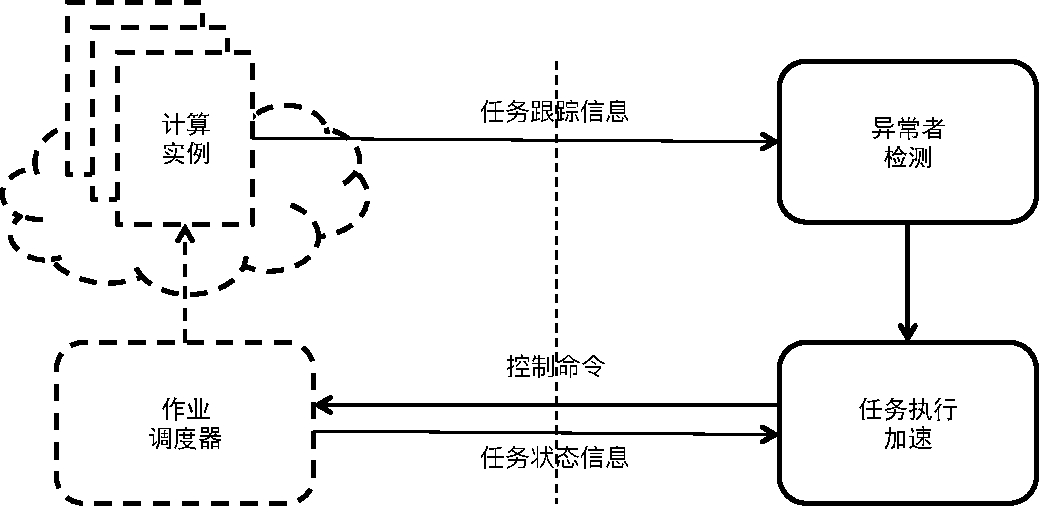
\includegraphics[width=0.8\textwidth]{NO2_arch.pdf}
  \caption{大规模并行任务加速器架构}
  \label{figure:no2arch}
\end{figure}

通过仔细设计接口,整个任务加速器保持了同作业调度器的独立性。这有利于用户根据自身需求选择不同的作业调度器。如图 \ref{figure:no2arch} 所示,任务加速器和 ProActive 作业调度器的接口部分只有获取一个作业的任务状态信息和发送任务管理命令。这些需求可以被任何作业调度器的控制接口满足。

下面将详细介绍系统的两个主要组成部分————异常者检测组件和任务执行加速组件。

\subsection{异常者检测}
\label{subsec:no2_trace}
异常者检测组件通过程序跟踪插桩工具和异常分析两个模块配合实现对大量并发任务中的异常者检测。如图 \ref{figure:tracing}所示,用户只需提供作业程序的二进制代码进行程序跟踪插桩,然后提交XML作业描述文件并使用插桩后的二进制代码作为执行文件。ProActive 作业调度器根据作业描述文件将计算任务分发到各个计算节点,各个节点执行插桩后的程序并返回任务执行进度跟踪信息给异常分析模块。异常分析模块利用聚类分析的手段找出潜在的异常者任务。
\begin{figure}
  \centering
  \includegraphics[width=0.85\textwidth]{NO2_tracing.pdf}
  \caption{程序跟踪插桩}
  \label{figure:tracing}
\end{figure}

异常者检测的实现基于对程序执行的跟踪和对跟踪信息的聚类分析。程序跟踪借助于静态二进制代码插桩实现,在 \ref{subsec:no2_inst} 节详细讨论了需要考虑的问题和主要方法。由于无法根据任务进度跟踪直接得出任务执行进度的准确信息,异常者分析模块的任务就是根据大量任务在执行过程中返回的进度跟踪信息判断是否有潜在异常者存在。在 \ref{subsec:no2_clustering} 节给出了基于机器学习中常用的聚类分析算法的一个简单、有效的发现异常者的方法。

\subsubsection{程序跟踪插桩工具}
\label{subsec:no2_inst}
在实际生产系统中使用二进制代码插桩跟踪程序的执行进度主要有两个挑战。一个挑战是性能开销,即使是轻量级的静态二进制插桩也可能带来数十个百分比的执行时间开销。另一个挑战是如何根据跟踪信息推测执行进度,这里的难点在于:1)在二进制代码中通过插桩工具埋下的程序跟踪点不是完全均匀一致的分布在整个执行过程中的;2)即使程序跟踪点在程序执行过程中均匀的被触发,仍然不能预测出任务已经完成了多少,还要执行多久。

以下载一个文件为例:如果下载进度条一分钟后显示已经完成了 50\%,很明显任务已经完成了一半并且在一个稳定的网络带宽下可能还需一分钟的时间。这就是数据密集型任务的进度预测的基本思路。但对于计算密集型任务来说,二进制程序插桩只能得到程序执行过程中触发了哪些插桩点的信息,无法得知程序执行的绝对进度。没有了类似数据密集型任务输入输出与执行进度相关的假设,计算密集型任务的执行进度很难通过二进制代码插桩进行预测。二进制代码插桩只能作为提供程序执行跟踪信息的手段,而实际上大量并发任务的异常者检测也不必非要预测任务的绝对执行进度。因此程序插桩工具只负责进行程序跟踪,异常者则交由异常者分析模块根据大量并发任务执行的跟踪信息分析得出。在本节我们重点讨论如何解决二进制代码插桩给程序执行带来的性能问题。

通过对多个计算密集型程序的二进制代码插桩和观察,可以得出两个发现:1)程序中不同的函数处在不同的调用层次;2)相同层次的函数被调用的频率相近,少数底层的函数被调用的极为频繁占用了大多数执行时间。表\ref{table:inst-stats}给出了插桩了全部函数入口点的 ImageMagick 动态链接库的函数调用次数统计信息。该函数库中有超过 1060 个函数,其中只有 33 个函数在多次执行中被调用超过 10000 次。
\begin{table}
\centering
\begin{threeparttable}
\caption{ImageMagick 函数调用信息统计}
\label{table:inst-stats}
\begin{tabular}{c|c|c}
\hline
调用次数 & 函数个数 & 函数举例 \\
\hline
above $10^7$ & 6 & CopyMagickMemory \\
$10^6$ - $10^7$ & 16 & GetCacheNexus \\
$10^5$ - $10^6$ & 2 & LocaleCompare \\
$10^4$ - $10^5$ & 9 & GetNexus \\
$10^3$ - $10^4$ & 10 & AddValueToSplayTree \\
$10^2$ - $10^3$ & 17 & FormatMagickStringList \\
$10^1$ - $10^2$ & 78 & NewSplayTree \\
$0$    - $10^1$ & 922 & GaussianBlurImage \\
\hline
\end{tabular}
\small 注:每个调用次数量级只给出一个函数作为例子。 
\end{threeparttable}
\end{table}

函数进入/退出点,和基本块(Basic Block)是常用的二进制代码的程序插桩点。理想的程序执行跟踪是对所有这些插桩点进行插桩,以实现更好的代码覆盖效果。然而,二进制代码程序插桩的开销明显是和埋下的插桩点数量成比例的。通过选择相对粗力度的插桩可以跳过少部分底层函数,从而去掉了大部分的插桩开销。为了能够准确跟踪程序执行,二进制代码的插桩需要足够的覆盖程度。如何在保证足够大范围的插桩覆盖的要求下达到最低的插桩开销?下面给出了基于函数调用次数统计的程序跟踪插桩方法。整个程序跟踪插桩的核心有两点:1)跟踪插桩点的选择;2)插桩点触发时执行的操作。

插桩点选择方法首先对二进制代码中的所有函数埋下插桩点,纪录每个函数的调用情况。然后多次执行插桩后的程序并统计函数调用次数信息。通过多次执行,不同调用层次的函数被区分开来。所有函数被调用次数的均值可以作为一个判断函数是否属于被频繁调用的底层函数的标准。所有大于这个均值的调用次数的函数,在最终的用于跟踪程序执行进度的插桩点选择中得以跳过。对于编程良好的程序,这样的自动插桩点选择方法可以同时保证足够大的执行进度跟踪覆盖和足够低的运行时开销。

在每个选定的程序插桩点可以插入一段代码,这段代码就是插桩点触发时需要执行的操作。对于程序执行的跟踪,在所有选定的函数入口进行插桩可以纪录下该函数调用的相关信息。由于这里程序跟踪的最终目标是在大量并发任务中检测潜在的异常者,在插桩点执行的操作可以简化为将一个插桩点计数器加一。这样就保证了在每个插桩点只有极低的运行开销。

\subsubsection{异常者分析}
\label{subsec:no2_clustering}
对于计算密集型并行任务的加速来说,第一个首要的目标是找出异常者。进行二进制插桩后的程序在各个节点执行,大量的并行任务运行中会提供程序的跟踪信息给异常者分析模块。虽然没有任务执行的绝对进度信息,通过比较所有并行任务的跟踪信息还是可以对潜在的异常者加以区分。这里使用统计分析和数据挖掘中常用的聚类分析方法对各个节点返回的程序跟踪信息进行聚类。对于大规模并行任务节点的程序跟踪信息的聚类分析基于如下假设:
\begin{itemize}
\item 在海量并行任务中,异常者只占较少的一部分。
\item 作业的分割基本保持均匀,即所有任务的规模大致相同。
\item 集群中的服务器节点异常以非确定的方式出现且过一段时间可能恢复正常。
\end{itemize}

异常者由于这样或者那样的原因执行缓慢,在程序跟踪的信息上同正常节点会表现出明显的(甚至是数量级上的)差距。这里使用大规模并行任务进度跟踪反馈的插桩点计数器信息提取每个任务的两个特征作为聚类依据,使用 K-means 聚类分析算法对正常节点和异常者加以区分。这两个特征分别是插桩点计数器累积值和最近一个程序跟踪信息反馈周期的插桩点计数器增量。它们基本反映了任务执行的进度和即时状态。图 \ref{figure:clusteringexample} 给出了一个基于这两个特征进行二类聚类分析的例子。
\begin{figure}
  \centering
  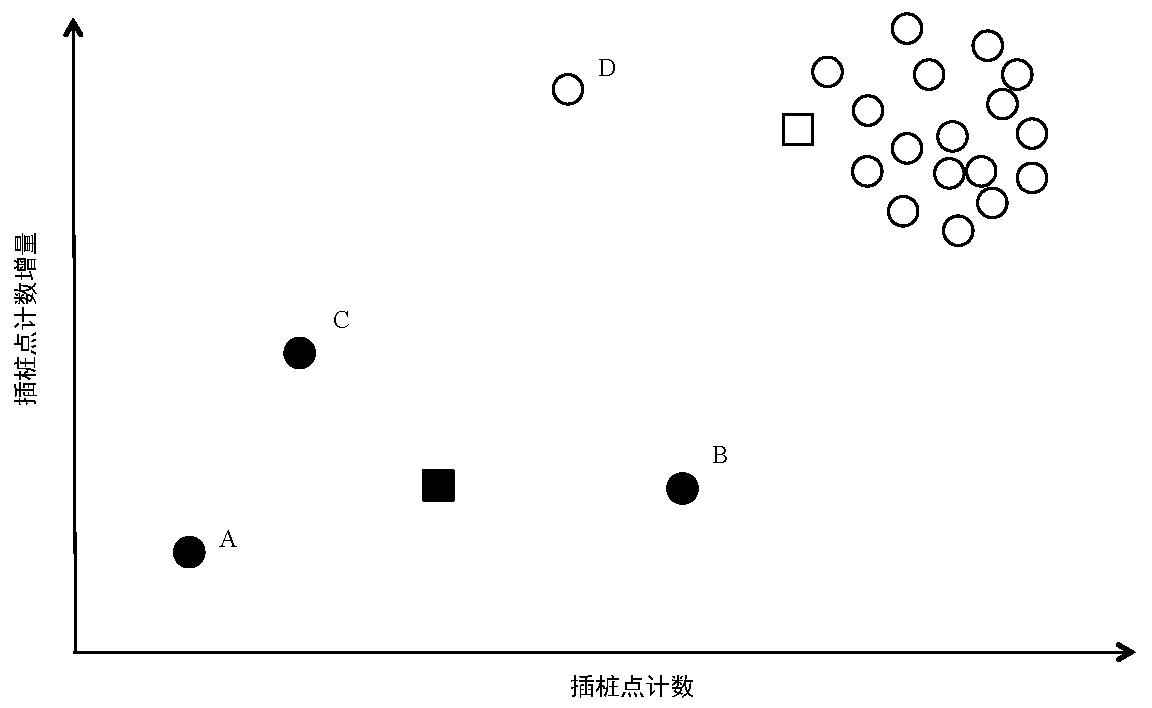
\includegraphics[width=0.8\textwidth]{clusteringexample.pdf}
  \caption{一个对并行任务程序跟踪信息使用K-means进行二类聚类分析的例子}
  \label{figure:clusteringexample}
\end{figure}

程序跟踪信息中插桩点计数器的值可用于在大量并发任务中比较相对的快慢,而最近一个反馈周期的插桩点计数增量体现的则是最近一小段时间某个任务的执行状态。单纯的使用插桩点计数器的值无法快速发现在任务执行过程中出现异常的节点,结合这两个参数可以在把握大量并发任务整体执行状态的同时迅速的找出可疑的异常者。如图 \ref{figure:clusteringexample} 所示,一个简单的 $k = 2$ 的 K-means 聚类可以大致将代表任务执行状态的点分为两类。从图 \ref{figure:clusteringexample} 中显然可以判断出,左下方的 $A$ 点和 $C$ 点极有可能代表异常者的任务状态。对于图 \ref{figure:clusteringexample} 中的 $B$ 点和 $D$ 点,只能认为它们有可能是异常者。对于异常者任务执行加速的目标来说,可以接受误报(False Positive),但不能接受漏报(False Negtive)。因为误报只会损失一些计算资源,而漏报则会直接贻误任务执行加速的时机进而影响作业完成时间。所以,在计算资源允许的情况下合理的策略是对所有潜在的异常者都通过备份执行实现容错。

\begin{algorithm}
\caption{异常者聚类}
\label{fig-outlier-algo}
\KwIn{$traces$}
\KwOut{$outliers$}%
$clusters\gets kmeans(traces, 2)$\;
$outliers\gets[]$\;
\If{$\left|clusters[1].centroid - clusters[2].centroid\right| \gg 0$}
{
  \uIf{$clusters[1].size \ll clusters[2].size$}
  {
    $outliers\gets [clusters[1], outlierClustering(clusters[2])]$
  }
  \ElseIf{$clusters[1].size \gg clusters[2].size$}
  {
    $outliers\gets [clusters[2], outlierClustering(clusters[1])]$
  }
}
\Return{$outliers$}
\end{algorithm}

算法 \ref{fig-outlier-algo} 给出了一个基于 K-means 聚类分析的异常者聚类方法。由于 K-means 算法对初值的选取比较敏感,而这里聚类的目标是将异常者任务和正常任务分成两类。因此可以用所有点中两个特征值的最小值作为一类初始聚类中心,所有点中两个特征值的最大值作为另一类初始聚类中心。如前文所述,异常者检测的目标是报告可疑的异常者。为了减少漏报,可以接受一定程度的误报。因此,在第一次 K-means 聚类后,可以对被认为不是异常者的一类再进行一次同样的 $k = 2$ 的 K-means 聚类分析,以过滤掉图 \ref{figure:clusteringexample} 中的类似 $D$ 点的情形。这样可以保证很大程度上的不漏报。

\subsection{任务执行加速}
在异常者检测组件给出了潜在异常者的情况下,可以利用竞价型实例低成本的执行一个和潜在异常者同样的任务。这样通过对同一个计算任务的投机执行,减轻了某个节点上可能的异常拖慢整体作业执行进度的程度。由于竞价型实例的申请和启动需要几分钟甚至十几分钟的时间,在发现潜在的异常者后再去申请竞价型实例显然就丧失了加速执行的机会。因此系统中需要维护一个竞价型实例资源池,这样在需要对计算任务增加一个执行副本时可以将竞价型实例立即投入使用。大规模并行计算任务运行在按需型实例组成的虚拟集群中,竞价型实例资源池负责提供需要投机执行时的计算资源。所有竞价型实例的竞价设定为市场价格,当市场价格升高实例被回收时则重新申请。如果竞价型实例市场价格超过了相应按需型实例的价格,则没有必要再使用竞价型实例计算资源加速按需型实例上的大规模并行计算任务。

\subsubsection{执行加速策略}
在某个节点可能存在异常的情况下,将其上执行的相同任务在其他节点冗余执行以期容错的机制这里称之为投机执行。当多个执行副本中的一个完成任务时,即可停止其他副本的执行。利用投机执行加速大规模并行任务在策略上有一些直观的经验规则:
\begin{enumerate}
\item 对进度最慢的异常者分配最高的投机执行优先级,显然这是加速作业完成的最优选择。
\item 尽早对潜在异常者发起投机执行。投机执行的目标是尽量减少作业完成时间,尽早执行意味着更好的提早完成的机会。
\item 针对某个异常者任务投机执行时,由于比其它任务开始的晚,为了加快执行速度在任务特点允许的情况下可以将该任务分成若干个子任务交由多个节点执行。
\end{enumerate}

当用户提交作业后,任务执行加速器作为一个守护进程运行在管理节点上。守护进程获取各个任务的程序跟踪信息的频率应该保证不影响ProActive作业管理器的正常执行。任务加速执行策略的主要部分如算法 \ref{fig-acc-algo} 所示,该算法定期的获取各个节点上执行的任务的程序跟踪反馈信息,通过聚类分析找出其中潜在的异常者。对于可能是异常者的任务,使用执行加速策略。对于投机执行的任务,一旦有一个任务副本执行完成,即可停止另一个副本的执行。如果该任务可进行拆分,算法 \ref{fig-acc-algo} 默认将任务拆分为两个子任务执行,在整个作业中已经有任务完成时将任务拆分为更多的子任务以减少任务完成所需时间。当然这要考虑作业的实际情况,在条件允许的情况下进行拆分。
\begin{algorithm}
\caption{执行加速}
\label{fig-acc-algo}
\KwIn{$job$ and sleep $interval$}
\KwOut{$job.state$}
$shards\gets 2$\;
\While{$job.state\not=FinishedOrFaulty$}
{
  \If{$job.finished\_tasks\not=nil$}
  {
    $shards\gets job.finsished\_tasks.size + 1$\;
  }
  $tasks\gets job.unfinished\_tasks$\;
  $outliers\gets outlierClustering(tasks.traces)$\;
  \ForEach{$outlier \in outliers$}
  {
    \If{$! outlier.task.replicated$}
    {
      \eIf{$outlier.task.divisible$}
      {
        $shards\gets min(shards, outlier.task.pieces)$\;
        $r\gets job\_submit(task\_split(outlier.task, shards))$\;
      }{
        $r\gets job\_submit(outlier.task)$\;
      }
      $replications\gets [replications, r]$\;
    }
  }
  $sleep(interval)$\;
  $job.update()$\;
  \For{$r \in replications$}
  {
    \uIf{$r.state = Finished$}
    {
      $kill(r.outlier.taskid)$\;
    }
    \ElseIf{$r.outlier.state = Finished$}
    {
      $kill(r.jobid)$\;
    }
  }
}
\KwRet{$job.state$};
\end{algorithm}

\subsubsection{计算资源利用率优化}
在发现潜在异常者后,除了使用竞价型实例进行针对性的双副本执行,还可以利用系统中空闲的按需型实例进行这样的冗余计算。这种情况可能出现在该节点已经执行完被分配的任务,但整个作业还没有完成的情况。联系算法 \ref{fig-acc-algo},随着部分节点完成任务后开始增加副本执行的任务拆分个数就是基于这一点考虑。

在用户提交作业后向各个节点分发任务前,由于还没有潜在异常者的出现竞价型实例将处于空闲状态。这部分空闲的计算资源也可以用来进行纯粹的``复制执行'',即在不知道各个节点状态的情况下冗余执行一些任务的副本。由于竞价型实例资源池一般小于按需计算实例的规模,因此投机执行只能针对部分节点。一个简单的策略是选择上次作业执行过程中出现的异常者节点,如果还有剩余的竞价型实例则可以随机指定。在作业开始执行后出现异常者时,如果恰好有对应的备份执行节点且正常则不用再投机执行该任务。如果没有对应的备份执行节点,可以停掉某个两个任务备份都正常执行的双副本中的竞价型实例上的任务副本用于提供给新出现的异常者做任务投机执行。

\section{系统实现}
\label{subsec:no2_impl}
为了更好的理解,本节对大规模计算密集型并行任务加速器中一些重要的实现细节加以解释。原型系统中使用的技术和一些背后的实现技巧也进行了简短地介绍。

二进制插桩部分基于DynInst \cite{Dyninst-Deconstruction} 插桩库的静态插桩实现。DynInst 是一个支持对二进制代码进行静态插桩,或对运行中的进程进行动态插桩的工具函数库。它提供了一个机器无关的构建插桩工具和应用的接口。插桩点选择部分对所有函数调用次数的统计基于DynInst的一个使用例程,CodeCoverage \cite{codecoverage}。
	
对于插桩点选择器,有三个代码片段(Code Snippet)插桩到程序中:初始化部分代码片段插桩到程序的开始,用于创建一些数据结构用于统计所需信息;最为常用的代码片段插桩到所有函数的入口点,用于纪录每一次函数调用;最后一个代码片段插桩到程序的结束,用于将函数统计信息保存到一个文件。同样有三个代码片段用于最终的任务进度跟踪插桩,初始化和结束部分用于申请和释放共享内存。最常用的代码片段负责将程序跟踪插桩计数加一。

任务加速器的投机执行部分基于 ProActive Scheduler \cite{pascheduling} 实现。通过控制脚本,任务加速器可以同ProActive的作业调度器进行交互。控制脚本是Javascript风格的语言,解释引擎基于集成于Java SE发行版的 Rhino \cite{Rhino:2016} 脚本引擎。通过控制脚本可以在运行时调用Java实现的ProActive作业调度器的对象和方法。

任务加速器根据异常者聚类结果选择需要进行投机执行的任务。对于每个异常者,生成一个紧急作业并给予一个根据异常者拖慢进度的程度确定的优先级。每个紧急作业可能包含一个或多个需要执行的任务,所有这些紧急作业按照投机优先级顺序提交给作业调度器。通过在作业描述中声明执行节点选择并提供节点选择脚本可以避免投机执行的任务被再次提交到一个异常节点。可以根据任务的大小选择调整异常者检测和执行加速的间隔,避免过于频繁的交互对作业调度器造成的干扰。程序跟踪信息只有插桩点的计数,所占用的内存和传输带宽非常小,对性能的影响可以忽略不计。

在整个实现中还提供了三个Shell脚本用于任务分割,本地代码封装,以及结果合并。Shell脚本将被提交给作业调度器作为正常作业执行。这实例上类似 MapReduce 任务的处理方式。用户只需增加具体的任务切分的命令到任务分割脚本中和一个收集结果的命令到结果合并脚本中,这对于一些作业可能是不必要的。一些默认的步骤,如:拷贝分割后的输入文件到任务执行节点,也可以根据具体情况进行修改。在本地代码封装脚本中,本地程序通过一条命令执行。用于传输任务跟踪信息的守护进程也在这个脚本中启动。用户可以极为灵活的使本地程序得以大规模并行。

为了更好的程序执行性能,程序的插桩部分使用共享内存将结果传递给传输任务进度跟踪信息的守护进程,通过对内存的读写实现了纪录程序跟踪数据的目的。这样每次程序执行过程中遇到插桩点时只引入了内存写操作,相对文件读写大大降低了性能开销。

\section{系统评测}
\label{sec:no2_eval}
通过一系列在云平台中展开的实验,本节给出了大规模计算密集型并行任务加速器的性能相关的评测结果。系统原型部署在 Amazon EC2 云平台的 ``us-east1'' 区域,使用 StarCluster \cite{starcluster} 将虚拟机计算实例组织成一个虚拟集群。StarCluster \cite{starcluster} 是一个 Amazon EC2 云平台上自动化虚拟集群构建、配置、管理的工具包,可以简化整个虚拟集群的部署过程。在虚拟集群中一个 EBS 被挂载在 Master 节点作为共享存储上以 NFS 文件系统的方式共享给集群中的所有节点。ProActive Scheduler 和本章的任务加速器部署在虚拟集群的 Master 节点上,虚拟集群中的虚拟机实例被以 SSH 架构类型节点资源的形式纳入到 ProActive 框架的管理调度中。虚拟集群中的计算资源包括 200 个按需型实例,以及在同一可用区维护的竞价型实例计算资源池。虚拟集群中所有虚拟机实例的配置类型选用 ``linux.m1.small'' 类型节点。该类型实例有 1.7 GB 内存和一个虚拟 CPU 核(约一个 EC2 运算单元的计算能力),存储块设备为 EBS。

实验中选用的代表性应用有两个:一个是生物信息学领域的 Cap3 \cite{Huang:1999:Cap3},另一个是影像处理中常用的 ImageMagick \cite{imagemagick}。Cap3 是生物信息学中比较常见的基因序列拼接组装程序,它的输入是许多FASTA格式 \cite{fasta} 的表达序列标签(Expressed Sequence Tag)文件。Cap3作业接受的输入是一些需要尝试进行序列拼接的FASTA文件,每个Cap3任务处理这样的一个或若干个文件。另一个应用 ImageMagick 是经典的开源影像处理工具,被广泛用于图像处理渲染等。其中的高斯模糊(Gaussian Blur)是一个常用的图像处理手段,在数学上看高斯模糊就是图像与正态分布(高斯分布)做卷积。高斯模糊能够减少图像中的噪点以及降低层次细节,常用于计算机视觉算法中的预先处理阶段,也被称为高斯平滑。实验中使用 Gaussian Blur 作为另一个应用案例,一个 Gaussian Blur 作业需要对大量的图片进行高斯模糊处理,每个任务需要处理一张或多张这样的图片。

评测中的第一个测试是针对程序跟踪带来的插桩性能开销的微基准测试,这关系到本章的任务执行加速器是否能用于实际的生产系统中。云平台的异常者情况也通过实验数据加以验证。系统评测中最主要的指标是作业完成时间,它直接反映出任务加速和性能提升的效果。另外,系统的计算资源使用率和一个长期的成本开销也是需要考虑的方面。

\subsection{程序插桩开销}
\label{sec:no2_overhead}
在任务加速器中,程序跟踪是异常者检测的基础。静态二进制代码插桩相比动态插桩的运行时开销已经小了很多,但如果对所有函数入口都埋入插桩点跟踪程序进度仍有不小的开销。这将使得任务加速器在异常者问题上的优化大打折扣甚至毫无意义。基于对程序执行过程中函数调用层次的观察,这里使用了一种基于采样的插桩点选择方法,在保证覆盖绝大多数函数的同时过滤掉了极少数调用频率特别高的函数,大大减少了程序跟踪插桩带来的开销。微基准测试集中对两个程序 Cap3 和 ImageMagick 使用两种不同的插桩方式得到的二进制代码在同一节点上执行,没有插桩的原始二进制代码作为基线也在相同节点上执行了同一任务。不同二进制代码的执行时间如图 \ref{figure:inst_overhead} 所示,插桩全部函数入口点在两个程序的执行中约带来 10\% 左右的运行时开销,而系统中使用的基于采样的程序跟踪插桩几乎和原始二进制代码执行时间相同,增加的运行时开销约0.1\%。

\begin{figure}
  \centering
  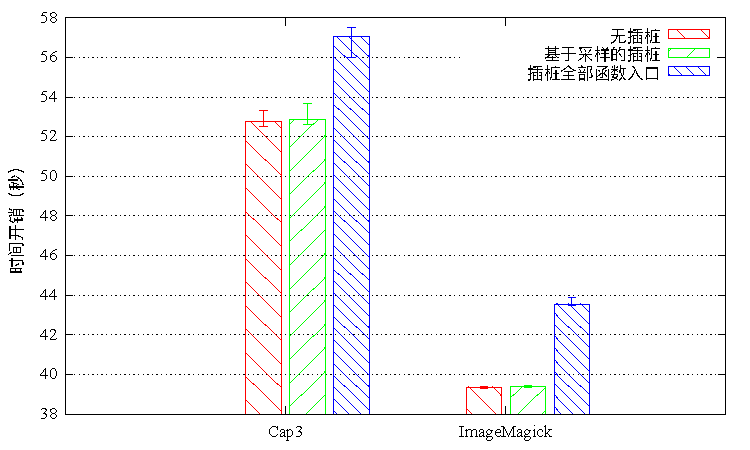
\includegraphics[width=0.9\textwidth]{inst_overhead.pdf}
  \caption{程序跟踪的插桩开销}
  \label{figure:inst_overhead}
\end{figure}

实验结果显示本系统使用的基于采样的程序跟踪插桩开销足够小,对程序的执行性能没有明显影响,可以用于大规模实际生产系统中。

\subsection{异常者情况}
云平台中异常者的现象在一个大规模虚拟集群中非常普遍,有些时候相对正常节点在I/O、网络性能上有明显下降。在其上运行的程序可能受到严重影响。为了测试虚拟集群中的异常者,这里向 ProActive 框架提交一个有100个相同任务的Cap3作业。在一天内不同阶段多次重复这个实验,可以发现异常者的情况有所区别,但很多时间段内都存在少量的明显慢于其它节点任务执行速度的节点存在。这里给出其中异常者较为严重的一次测试结果,具体如图 \ref{figure:outlier_cloud} 所示。
\begin{figure}
  \centering
  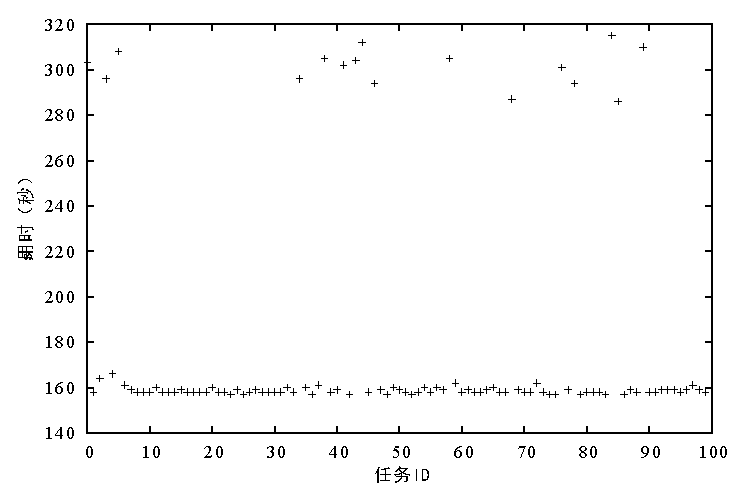
\includegraphics[width=0.8\textwidth]{cloud_outliers.eps}
  \caption{Amazon EC2云平台中100个节点在一次运行Cap3作业时的任务完成时间}
  \label{figure:outlier_cloud}
\end{figure}

从图 \ref{figure:outlier_cloud} 中可以看出,异常者可能导致整个作业被拖慢两倍甚至更长的时间。当虚拟集群中节点数量可观时出现异常者的情况变得常见。一个针对大规模并行任务集群的日志统计结果 \cite{Ananthanarayanan:2010:ROM:1924943.1924962} 显示有 25\% 的作业中有超过 15\% 的异常者出现。对于大规模并行计算任务来说,考虑异常者对整体作业进度的影响十分必要。

\subsection{性能改进}
\label{sec:no2_perf}
性能测试使用了虚拟集群中的200个按需计算实例,利用竞价型实例作为执行加速的廉价计算资源。在实验过程中,通过向 ProActive Scheduler 提交包含 200 个任务的 Cap3 作业或 GaussianBlur 作业测试了在不使用本章提出的任务加速器、使用本章任务加速器但不使用初始阶段的任务克隆策略,以及同时使用投机执行策略和任务克隆策略三种系统配置下的作业处理性能。测试中所使用的作业任务规模大小接近:Cap3 任务为对一个FASTA格式文件中的基因序列进行拼接,不可继续进行分割;GaussianBlur 任务为对一张图片进行高斯模糊处理,根据实际计算中的近似算法可继续分割。

竞价型实例计算资源池中的节点数量可以综合考虑成本因素,以及短期内异常者出现比率设定。用于消除异常者影响的竞价型实例数量不足可能导致有异常者没有对应的执行副本,最终仍拖慢作业完成进度。因此,在性能测试中首先要确定的是竞价型实例计算资源池中所需的节点数量。在一段时间内,针对两个应用分别尝试提供占所有按需型实例数量(本实验中为200个)不同百分比的竞价型实例数用于投机执行,在这个测试中不引入完成自身任务的空闲按需型实例进行投机执行。测得的作业完成时间如图 \ref{figure:replica_cap} 所示,在 Cap3 作业中有 9\%(18个)的竞价型实例用于投机执行就很好的抑制了异常者造成的影响,在 Gaussian 作业中则需要至少 24 个节点用于投机执行才起到减少作业完成时间的效果。这是因为 GaussianBlur 任务可以进行再次拆分,每次投机执行都会使用更多的计算节点。在用于投机执行的节点数达到 18\% 之后基本起到了消除异常者的效果,GaussianBlur 作业通过对任务拆分加快了任务执行进一步减少了作业完成时间,从而得到了比 Cap3 作业更好的性能提升。根据上述测试结果,接下来的性能测试中在竞价型实例资源池中维护 18\%(36个)的计算资源。为保证测试数据的准确性,在一段时间内相同的实验被重复多次,最后的结果取平均值和最小、最大值。实验结果如图 \ref{figure:completiontime_cloud} 所示。
\begin{figure}
  \centering
  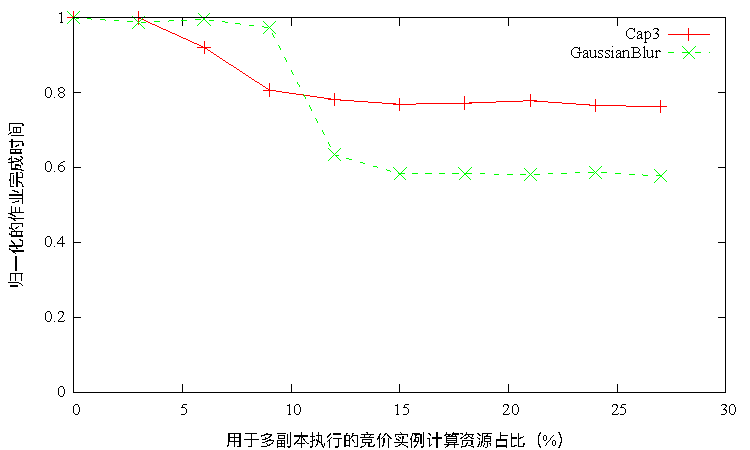
\includegraphics[width=0.9\textwidth]{replica_cap.pdf}
  \caption{用于投机执行的竞价型实例数同作业完成时间的关系}
  \label{figure:replica_cap}
\end{figure}

作业完成时间完全由执行最慢的任务决定。从图 \ref{figure:completiontime_cloud} 中可以看出,实验中作为基线的不使用任务加速器的 ProActive 框架的平均作业完成时间远远大于最好情况下的作业完成时间,这说明在大规模并行任务执行中异常者对整体作业执行带来的拖慢影响十分严重。在使用了投机执行策略后,Cap3 作业的平均完成时间被有效缩减了超过 20\%。由于 Cap3 任务不可继续分割,投机执行策略无法通过再次分割任务的方式加快任务执行。实验结果上看,在投机执行策略下 Cap3 作业的平均完成时间同没有异常者的最好情况仍有一段差距。因为,在发现异常者时副本执行的任务已经落后于正常节点。GaussianBlur 作业的平均执行时间在使用投机执行策略后将作业完成时间缩减了超过 40\%,接近作业执行时间的最好情况,基本消除了异常者带来的影响。这是因为虽然发现异常者时已经落后于正常节点,GaussianBlur 任务可以通过进一步分割减少完成任务所需的时间。如图 \ref{figure:completiontime_cloud} 所示,在任务初始阶段的任务克隆策略只在 Cap3 作业执行中带来了少量的性能提升,对于 GaussianBlur 作业则没有明显效果。虽然任务初始阶段的投机执行有潜在的性能优化机会,但由于异常者出现的不确定和偶发性其所能带来的性能提升在实验中并不明显。在任务不可分割的情况下,能一定程度上进一步减少异常者造成的拖慢作业完成时间影响。
\begin{figure}
  \centering
  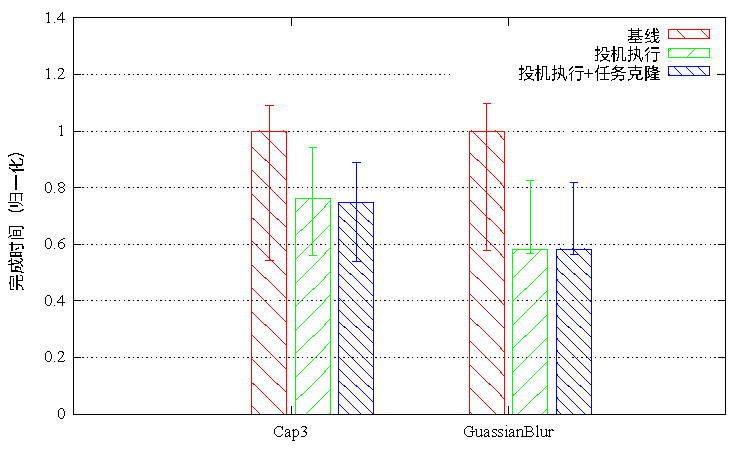
\includegraphics[width=0.9\textwidth]{cloud_completiontime.pdf}
  \caption{虚拟集群中的ProActive作业完成时间比较}
  \label{figure:completiontime_cloud}
\end{figure}

\subsection{资源使用率与成本开销}
\label{sec:no2_usage}
在进行性能测试的同时,ProActive Resource Manager 统计的CPU使用率也能一定程度上反映作业执行的效率。如图 \ref{figure:resourceusage_cloud} 所示,在大规模并行任务执行过程中,异常者不仅拖慢了整体作业完成进度还造成了一定的计算资源的空闲和浪费。在两个作业的执行中,均只有不到 50\% 左右的CPU使用率。使用投机执行和初始阶段任务克隆的策略,加快了作业完成进度,减少了计算资源的空闲时间。在任务可再次分割的情况下,更是能够充分利用已经完成任务执行的空闲节点计算资源。投机执行策略使 Cap3 作业的执行中 CPU 使用率增加到了约 70\%,在 Gaussian 作业中CPU使用率更是接近 90\%。
\begin{figure}
  \centering
  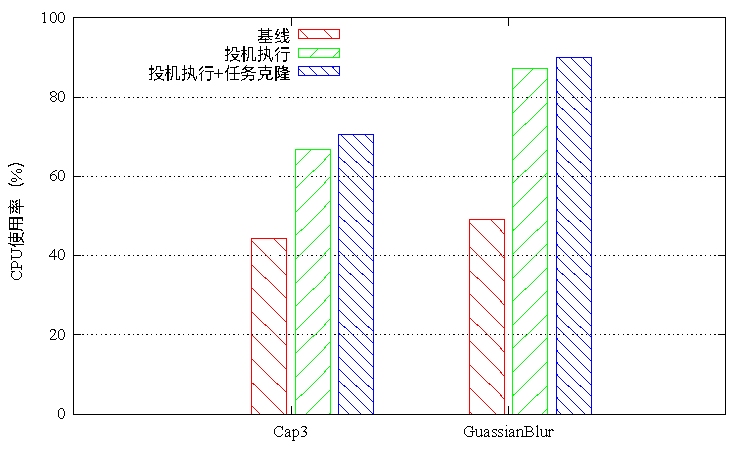
\includegraphics[width=0.9\textwidth]{cloud_usage.pdf}
  \caption{虚拟集群在ProActive作业执行中的CPU使用率比较}
  \label{figure:resourceusage_cloud}
\end{figure}

在计算成本开销方面,从长期的 Amazon EC2 云平台竞价型实例市场价格的历史数据看,竞价型实例的成本约为相同类型的按需成本的五分之一到十分之一。以本实验中使用的``linux.m1.small'' 类型来说,对于一个有200个按需计算实例的虚拟集群来说,36个竞价型实例的计算成本只有虚拟集群成本的约 3\%。

\section{本章讨论}
本章详细介绍了利用竞价型实例加速大规模计算密集型并行任务的方法,基于程序跟踪和聚类分析等手段实现了对海量并发计算密集型任务中的异常者的早期检测,通过投机执行等策略实现了作业完成时间的缩减,消除了异常者造成的影响。该方法的有效性在系统评测中得到了验证,但在实际应用中仍有一些需要注意的地方。

\subsection{对竞价节点的使用}
本章提出的大规模计算密集型并行任务处理加速方法,解决的是云平台虚拟集群中偶发性的节点异常拖慢作业完成进而影响工作流进度的问题。需要强调的是对竞价型实例的使用,本章的工作中将竞价型实例只用于投机执行等加速策略因而隔离了竞价节点失效对系统可靠性的影响。简单地将虚拟集群中的按需型实例全部或者部分换成同样成本但数量更多的竞价型实例似乎能进一步提升系统并发能力,实则不可行。云平台异常者的产生多种多样,包括:硬件故障、软件配置错误、共享I/O和网络带宽资源导致的竞争等。竞价节点潜在的不可靠性引入了一种新的节点异常,但这类异常完全不同于其它:1)竞价节点失效不是性能变差而是直接停机;2)竞价节点的异常不是偶发性、少量的,大量同一可用区竞价型实例的失效是强相关的。这同本章介绍的任务加速方法假设的系统中的异常者只占很少一部分相违背。而针对大量的节点异常使用投机执行策略时,大量新的执行副本同样面临执行过程中的异常者问题。事实上,这是另一个问题,即:在使用竞价型实例执行计算任务时如何处理竞价不足的节点失效问题。

\subsection{成本收益分析}
对于本章要解决的问题,一个十分简单的处理方法是更加激进的使用复制执行策略。在全部任务开始执行的时候直接进行冗余执行,每个任务有两个副本来消除异常者带来的影响。相对带来的性能提升,无论是使用按需型实例还是竞价型实例作为执行副本的计算资源都是不划算的。再考虑异常者长期的出现频率,使用一定比例的按需型实例作为执行副本的计算资源仍是一个很高的成本。相对应的,极为低廉的价格以及作为备用执行副本不要求可靠性的用途让竞价型实例成为了加速异常者的最佳选择。

\section{本章小节}
同以往的工作不同,本章提出了利用竞价型实例解决大规模计算密集型并行任务的异常者拖慢作业进度的低成本方法。该方法的原型实现在 ProActive 框架上,引入了针对大规模计算密集型任务的异常者检测方法。该方法通过组合基于二进制插桩的程序跟踪技术和基于聚类分析的异常者分析方法实现了对异常者的早期发现。在程序跟踪方面,通过基于采样的插桩点选择方法在保证足够覆盖性的前提下将插桩的运行时开销从 10\% 降低到了 约 0.1\%。投机执行和任务克隆等策略一定程度上消除了异常者的影响,针对任务可继续分割的情况通过使用多个节点完成一个异常者任务加速进一步减少了作业完成时间。针对两个典型应用的评测结果显示本章的工作实现了对大规模计算密集型任务的加速,大大减轻了异常者的影响。作业完成时间的缩减在两个应用中分别超过 20\% 和 40\%,而计算成本的增加只有约 3\%。


%%% 其它部分
\backmatter

%% 本科生要这几个索引,研究生不要。选择性留下。
% 插图索引
%\listoffigures
% 表格索引
%\listoftables
% 公式索引
%\listofequations


%% 参考文献
% 注意:至少需要引用一篇参考文献,否则下面两行可能引起编译错误。
% 如果不需要参考文献,请将下面两行删除或注释掉。
\bibliographystyle{thuthesis}
\bibliography{ref/refs}


%% 致谢
% 如果使用声明扫描页,将可选参数指定为扫描后的 PDF 文件名,例如:
% \begin{ack}[scan-statement.pdf]
\begin{acknowledgement}
衷心感谢导师郑纬民教授、武永卫教授引领我进入计算机系统研究的世界,在学术和生活上的指导和帮助为学生的成长提供了广阔的发展空间。衷心感谢陈康副教授一次次斧正我的想法和研究思路,每一次讨论都让我受益匪浅有 ``一语惊醒梦中人'' 之感。

在清华大学计算机系高性能计算研究所的学习与研究中,多年来承蒙杨广文教授、姜进磊副教授、薛巍副教授的关怀与帮助,不胜感激。

感谢以往论文的合作者、曾与我同在清华大学计算机系学习的任晶磊博士、赵勋博士、冯欢同学,从论文思路讨论到英文写作技巧都让我收获良多。感谢清华大学计算机系的博士研究生胡勇、高品、章明星、帝国理工大学计算机系的博士研究生郭策等同学在以往研究工作中给出的宝贵意见和建议。

感谢清华大学计算机系 MADSYS 组的全体同学,与优秀的各位一同学习、工作,交流学术与思想是我在研究生期间能快速成长的一大助力。

感谢清华大学计算机系的甘霖、苏茂萌、苏文博等与我一同入学的同学在课程学习直至学位论文撰写过程中的交流分享。

感谢 \thuthesis,它的存在让我的论文写作轻松自在了许多,让我的论文格式规整漂亮了许多。

最后,特别感谢我的父亲母亲对我一如既往的支持,这是我的学位论文能够成文不可或缺的精神力量;感谢我的女朋友对我的鼓励,携手在清华园求学是我今生最难忘的一段时光,来自完全不同领域的学术交流也开阔了我的研究思路和视野。

\end{acknowledgement}


%% 附录
\begin{appendix}
\chapter{论文相关证明}

\section{竞价实例市场价格的统计推断}

\end{appendix}

%% 个人简历
\begin{resume}

  \resumeitem{个人简历}

  1989 年 5 月 21 日出生于 黑龙江 省 青冈 县。

  2007 年 9 月考入 哈尔滨工业 大学 软件 学院 软件工程 专业,2011 年 7 月本科毕业并获得 工学 学士学位。

  2011 年 9 月免试进入 清华 大学 计算机 系攻读 博士 学位至今。

  \researchitem{发表的学术论文} % 发表的和录用的合在一起

  % 1. 已经刊载的学术论文(本人是第一作者,或者导师为第一作者本人是第二作者)
  \begin{publications}
    \item Yang Y, Ren T L, Zhang L T, et al. Miniature microphone with silicon-
      based ferroelectric thin films. Integrated Ferroelectrics, 2003,
      52:229-235. (SCI 收录, 检索号:758FZ.)
    \item 杨轶, 张宁欣, 任天令, 等. 硅基铁电微声学器件中薄膜残余应力的研究. 中国机
      械工程, 2005, 16(14):1289-1291. (EI 收录, 检索号:0534931 2907.)
    \item 杨轶, 张宁欣, 任天令, 等. 集成铁电器件中的关键工艺研究. 仪器仪表学报,
      2003, 24(S4):192-193. (EI 源刊.)
  \end{publications}

  % 2. 尚未刊载,但已经接到正式录用函的学术论文(本人为第一作者,或者
  %    导师为第一作者本人是第二作者)。
  \begin{publications}[before=\publicationskip,after=\publicationskip]
    \item Yang Y, Ren T L, Zhu Y P, et al. PMUTs for handwriting recognition. In
      press. (已被 Integrated Ferroelectrics 录用. SCI 源刊.)
  \end{publications}

  % 3. 其他学术论文。可列出除上述两种情况以外的其他学术论文,但必须是
  %    已经刊载或者收到正式录用函的论文。
  \begin{publications}
    \item Wu X M, Yang Y, Cai J, et al. Measurements of ferroelectric MEMS
      microphones. Integrated Ferroelectrics, 2005, 69:417-429. (SCI 收录, 检索号
      :896KM)
    \item 贾泽, 杨轶, 陈兢, 等. 用于压电和电容微麦克风的体硅腐蚀相关研究. 压电与声
      光, 2006, 28(1):117-119. (EI 收录, 检索号:06129773469)
    \item 伍晓明, 杨轶, 张宁欣, 等. 基于MEMS技术的集成铁电硅微麦克风. 中国集成电路,
      2003, 53:59-61.
  \end{publications}

  \researchitem{研究成果} % 有就写,没有就删除
  \begin{achievements}
    \item 任天令, 杨轶, 朱一平, 等. 硅基铁电微声学传感器畴极化区域控制和电极连接的
      方法: 中国, CN1602118A. (中国专利公开号)
    \item Ren T L, Yang Y, Zhu Y P, et al. Piezoelectric micro acoustic sensor
      based on ferroelectric materials: USA, No.11/215, 102. (美国发明专利申请号)
  \end{achievements}

\end{resume}

\end{document}
